%% INTRO SPIV

\chapter{Quarters} %DCG 11.
    \label{sec:upright}
    \oldlabel{3}

This chapter contains the technical heart of the proof of the Kepler
conjecture.  Its primary purpose is to obtain good bounds on the
score $\sigma_R(D)$ when $R$ is an arbitrary standard region of a
centered packing $D$.  This is particularly challenging, because
we have no {\it a priori} restrictions on the combinatorial type
of the standard region $R$.  It is not known to be bounded by a
simple polygon.  It is not known to be simply connected. Moreover,
there are multitudes of possible geometrical configurations of
upright and flat quarters, each scored by a different rule.  This
paper will deal with these complexities and will bound the score
$\sigma_R(D)$ in a way that depends on a simple numerical
invariant $n(R)$ of $R$. When $R$ is bounded by a simple polygon,
the numerical invariant is simply the number of sides of the
polygon. This bound on the score of a standard region represents
the turning point of the proof, in the sense that it caps the
complexity of a contravening centered packing, and restrains the
combinatorial possibilities. Later in the proof, it will be
instrumental in the complete enumeration of the planar hypermaps
attached to contravening stars.

The first section will prove a series of approximations for the
score of upright quarters.  The strategy is to limit the number of
geometrical configurations of upright quarters by showing that a
common upper bound (to the scoring function) can be found for
quite disparate geometrical configurations of upright quarters.
When a general upper bound can be found that is independent of the
geometrical details of upright quarters, we say that the upright
quarters can be {\it erased.}  (A precise definition of what it
means to erase an upright quarter appears below.)  There are some
upright quarters that cannot be treated in this manner; and this
adds some complications to the proofs in this paper

The second section states the main result of the paper
(Theorem~\ref{thm:the-main-theorem}).  An initial reduction
reduces the proof to the case that the boundary of the given
standard region is a polygon.  A further argument is presented to
reduce the proof to a convex polygon.

The third section completes the proof of the main theorem.  This
part of the proof relies on a new geometrical decomposition of the
part of a $V$-cell over a standard region. The pieces in this
decomposition are called {\it truncated corner cells}.

A final section in this paper collects miscellaneous further
bounds that will be needed in later parts of the proof of the
Kepler conjecture.






\section{Erasing Upright Quarters} %DCG 11.1,p.112
    \oldlabel{3.1}

\begin{definition}
A standard region is said to be {\it exceptional\/} if it is not a
triangle or a quadrilateral.  The pair $(D,R)$ consisting of a
centered packing and an exceptional standard region is said to be
an {\it exceptional cluster}.  The vertices of the packing of
height at most $2t_0$ that are contained in the closed cone over
the standard region are called its {\it corners}.
\end{definition}

Fix an exceptional cluster $R$. 

In Section~\ref{sec:upright}, we discuss how to eliminate many
cases of upright diagonals. The results are summarized in
Section~\ref{x-3.10}.

If $R$ is a standard region, we write $V_R(t)$ for the
intersection of the local $V$-cell $V_R = \op{VC}(0)\cap C(R)$
with a ball $B(t)$, centered at the origin, of radius $t$.  We
usually take $t=t_0$. If $\{0,v\}$, of length between $2t_0$ and
$2\sqrt{2}$, is not the diagonal of an upright quarter in the
$Q$-system, then $v$ does not affect the truncated cell $V_R(t_0)$
and may be disregarded. For this reason we confine our attention
to upright diagonals that lie along an upright quarter in the
$Q$-system.

%\section{Truncation}
    \oldlabel{3.2}

%% XX Clean this up. What if something is masked?
%% In fact, just get rid of "erasing" It is so messy.

We say that an upright diagonal $\{0,v\}$ can be {\it erased with
penalty $\pi_0\ge0$}, if we have, in terms of the  decomposition
of \Chap~\ref{sec:fine},
    $$
    \sum_Q\sigma(Q) +\sum_S\sigma(V_S(t_S)) - 4\doct\sum_W\op{vol}(\bigd(v,W))<
        \pi_0+\sum_Q\svor_0(Q) +\sum_S\svor_0(S).
    $$
Here the sum over $Q$ runs over the upright quarters around
$\{0,v\}$. The scores $\sigma(Q)$ are context-dependent (see
Section~\ref{sec:scoring}). The second sum runs over simplices $S$
along $\{0,v\}$ of type $\SC$ in the $\CalS$-system.  We define
their score $\sigma(V_S(t_S))$ as in \Chap~\ref{sec:fine}. Also,
$\bigd(v,W)$ is the piece of the decomposition of Definition~\ref{def:delta-a}. 
The right-hand side is scored by the
truncation function in \Chap~\ref{sec:scoring}
Formula~\ref{eqn:3.7}. When we erase without mention of a penalty,
$\pi_0=0$ is assumed.

If the diagonal can be erased, an upper bound on the score is
obtained by ignoring the upright diagonal and all of the
structures around it coming from the decomposition of
\Chap~\ref{sec:fine}, and switching to the truncation at $t_0$.
Section~\ref{x-3} shows that various vertices can be erased, and
this will greatly reduce the number combinatorial possibilities
for an exceptional cluster.

\section{Contexts} %DCG 11.2, p.113
    \oldlabel{3.3}

Each upright diagonal has a context $\x(p,q)$, with $p$ the number
of anchors and $p-q$ the number of quarters around the diagonal
(Definition~\ref{def:context}). The dihedral angle of a quarter is
less than\footnote{\calc{971555266}} $\pi$, so the context
$\x(2,0)$ is impossible. There is at least one quarter, so $p\ge
q+1$, $p\ge2$.

The context $\x(2,1)$ is treated in Section~\ref{sec:bounds}.
Lemma~\ref{lemma:mixed-vor0} shows that by removing the upright
diagonal, and scoring the surrounding region by a truncated
function $\vor_0$, an upper bound on the score is obtained. In the
remaining contexts, $p\ge3$. We start with contexts satisfying
$p=3$. The context $\x(3,0)$ is to be regarded as two
quasi-regular tetrahedra sharing a face rather than as three
quarters along a diagonal.  In particular, by
Definition~\ref{def:q-system}, the upright quarters do not belong
to the $Q$-system.

We recall that 
$$\sigma(Q,v)=\nu(Q,v)$$
where $\nu(Q,v)$ is given in Definition~\ref{def:nu},
where $Q$ is any upright quarter in the $Q$-system, except for
contexts $\x(2,1)$ and $\x(4,0)$.
The
context $\x(2,1)$ has been treated, and the context $\x(4,0)$ does
not occur in exceptional clusters. Thus, for the remainder of this
\chap, the scoring rule $\sigma(Q,v)=\nu(Q,v)$ will be used.



We have several different variants on the score depending on the
truncation, analytic continuation, and so forth.  If $f$ is any of the
functions
    $$\svor_0,\ \svor,\ \Gamma, \ \nu,$$
we set $\tau_{0}$, $\tau_V$, $\tau_\Gamma$,
$\tau_\nu$, respectively,
to
    $$\tau_* = -f(S) +\sol(S)\zeta\pt.$$
We set
    $\tau(S,t) = -\svor(S,t)+\sol(S)\zeta\pt$.
The family of functions $\tau_*$ measure what is squandered by a
simplex.  We say that $Q$ is compressed or decompressed 
according to the scoring of $\mu(Q)$.  (See
Section~\ref{sec:rules}.)




\section{Three anchors} %DCG 11.3,p.114
    \oldlabel{3.4}


\begin{lemma}
    \oldlabel{3.4.1}
The upright diagonal can be erased in the context $\x(3,2)$.
\end{lemma}


\begin{proof}
Let $v_1$ and $v_2$ be the two anchors of the upright diagonal $\{0,v\}$
along the quarter. Let the third anchor be $v_3$.

Assume first that $|v|\ge 2.696$. If $Q$ is compressed,
then\footnote{\calc{73974037}} %A10  by $\A_{10}$,
the score is dominated by the truncated
function $\svor_0$.  Assume $Q$ is decompressed. If $|v_1|$,
$|v_2|\le 2.45$, then a calculation\footnote{\calc{764978100}} %A11
gives the result. Take $|v_2|\ge
2.45$.  By symmetry, $|v-v_1|$ or $|v-v_2|\ge 2.45$. The case
$|v-v_1|\ge2.45$ is treated by another calculation.%
\footnote{\calc{764978100}} %A11
We take
$|v-v_2|\ge2.45$. Let $S=\{0,v,v_2,v_3\}$. If $S$ is of type $\SC$,
the result follows.\footnote{\calc{764978100}} %A11
$S$ is of type $\SC$, if and only if $y_4\le 2.77$, (because
by Lemma~\ref{tarski:eta245}, $\eta_{456}>\sqrt2$).
If $S$ is  not of type $\SC$, then by Lemma~\ref{tarski:eta696} and
Lemma~\ref{tarski:eta-rad},
we have $\rad(S) \ge\eta(|v|,2.45,24.5)\ge \eta_0(|v|/2)$.
This justifies the use of $\kappa$ (see Section~\ref{x-2.3}
Case (2)). That the truncated function dominates the score now
follows from a calculation.\footnote{\calc{618205535}} %A9

Now assume that $|v|\le 2.696$. If the simplices $\{0,v,v_1,v_3\}$
and $\{0,v,v_2,v_3\}$ are of type $\SC$, the bound follows from a
calculation.\footnote{\calc{73974037}} %A10
\footnote{\calc{764978100}} %A11
%$\A_{10},\A_{11}$.
If say  $S=\{0,v,v_2,v_3\}$ is not of type $\SC$,
then
    $$\rad(S)\ge\sqrt2>  \eta_0(2.696/2)\ge\eta_0(h),$$
justifying the use of $\kappa$. The bound follows from further
calculations.\footnote{\calc{618205535}} %A9
\footnote{\calc{73974037}} %A10
\footnote{\calc{764978100}} %A11
%    $\A_9,\A_{10},\A_{11}$.
($\Gamma+\kappa <\octavor_0$,
etc.)
\end{proof}

\begin{lemma}
    \oldlabel{3.4.2}
    \label{lemma:unerased}
The upright diagonal can be erased in the context $\x(3,1)$, provided
the three anchors do not form a flat quarter at the origin.
\end{lemma}

\begin{proof}
In the absence of a flat quarter, truncate, score, and remove the
vertex $v$ as in the context $\x(3,1)$ of
Lemma~\ref{lemma:mixed-vor0}. If there is a flat quarter, by the
rules of Definition~\ref{def:q-system}, $v$ is enclosed over the
flat quarter. We do nothing further with them for now. This
unerased case appears in the summary at the end of the
section~(\ref{x-3.10}).  See Lemma~\ref{lemma:min0-svor}.
\end{proof}

\section{Six anchors} %DCG 11.4, p.115
    \oldlabel{3.5}

\begin{lemma}  An upright diagonal has at most five anchors.
\end{lemma}

\begin{proof}
The proof relies on constants and inequalities from two
calculations.\footnote{\calc{729988292}} %A3
\footnote{\calc{83777706}} %A8
%$\A_3$ and $\A_8$.
If between two anchors there is a quarter, then the angle is
greater than $0.956$, but if there is not,  the angle is greater than
$1.23$.  So if there are $k$ quarters and at least six anchors, they
squander more than
    $$ k (1.01104) - [2\pi-(6-k)1.23]0.78701 > \squander,$$
for $k\ge0$.
\end{proof}

\section{Anchored simplices} %DCG 11.5,p.115
    \oldlabel{3.6}
    \label{sec:anchored-simplex}

Let $\{0,v\}$ be an upright diagonal, and let
$v_1,v_2,\ldots,v_k=v_1$ be its anchors, ordered cyclically around
$\{0,v\}$.  This cyclic order gives dihedral angles between
consecutive anchors around the upright diagonal. We define the
dihedral angles so that their sum is $2\pi$, even though this will
lead us to depart from our usual conventions by assigning a
dihedral angle greater than $\pi$ when all the anchors are
concentrated in some half-space bounded by a plane through
$\{0,v\}$. When the dihedral angle of $S=\{0,v,v_i,v_{i+1}\}$ is at
most $\pi$, we say that $S$ is an {\it anchored simplex\/} if
$|v_i-v_{i+1}|\le3.2$. (The constant $3.2$ appears throughout this
\chap.) All upright quarters are anchored simplices. If an upright
diagonal is completely surrounded by anchored simplices, the
upright diagonal is sometimes called a {\it loop}. If
$|v_i-v_{i+1}|>3.2$ and the angle is less than $\pi$, we say there
is a {\it large gap\/} around $\{0,v\}$ between $v_i$ and $v_{i+1}$.

To understand how the interiors of anchored simplices meet, we
need a bound satisfied by vertices enclosed over an anchored
simplex.

\begin{lemma}
    \label{lemma:anc-simplex-not-enc}
A vertex $w$ of height between 2 and $2\sqrt{2}$, enclosed in the cone
over an anchored simplex $\{0,v,v_1,v_2\}$ with diagonal $\{0,v\}$ satisfies
$|w-v|\le 2t_0$. In particular, if $|w|\le 2t_0$, then $w$ is an anchor.
\end{lemma}

\begin{proof}
This appears as Lemma~\ref{tarski:anc-simplex-not-enc}.
\end{proof}


\begin{corollary}
A vertex of height at most $2t_0$ is never enclosed over an anchored
simplex.
\end{corollary}

\begin{proof}  If so, it would be an anchor to the upright diagonal, contrary to
the assumption that the anchored simplex is formed by consecutive
anchors.
\end{proof}


\section{Anchored simplices do not overlap} %DCG 11.6, p.116
    \oldlabel{3.7}



\begin{definition}\index{unconfined@3-unconfined}
 \index{crowded4@3-crowded}\index{crowded3@4-crowded}
% Def'n copied from linprog.tex
Consider an upright diagonal that is not a loop. Let $R$ be the
standard region that contains the upright diagonal and its
surrounding quarters.  Assume we are in the context $(4,1)$ or
$(5,1)$.  In the context $(4,1)$, suppose that there does not exist
a plane through the upright diagonal such that all three quarters
lie in the same half-space bounded by the plane. Then we say that
the context is {\it $3$-unconfined}. If such a plane exists, we say
that the context is $3$-crowded. We call the context $(5,1)$ a
$4$-crowded upright diagonal. Sections~\ref{x-3.4} and \ref{x-3.5}
reduce everything to contexts with four or five anchors around each
vertex.  If there are $5$ anchors, Lemma~\ref{x-3.8.1} (and
Remark~\ref{rem:2gap}) show that we can assume at most one large
gap. This gives contexts $(5,0)$ and $(5,1)$.  If there are four
anchors, then Lemma~\ref{x-3.9.1} will dismiss all contexts except
$(4,0)$ and $(4,1)$. Thus, every upright diagonal is exactly one of
the following: a loop, $3$-unconfined, $3$-crowded, or $4$-crowded.
%\def\Sfour{{{\cal\mathbf S}_4^+}}  --> $4$-crowded upright diagonal
%\def\Sminus{{{\cal\mathbf S}_3^-}} --> $3$-crowded upright diagonal
%\def\Splus{{{\cal\mathbf S}_3^+}}  --> $3$-unconfined upright diagonal
\end{definition}


This lemma is a consequence of the two others that follow. The
context of the lemma is the set of anchored simplices that have
not been erased by previous reductions.

\begin{lemma}
    \label{lemma:anchor-no-overlap}
The interiors of anchored simplices do not meet.
\end{lemma}

The remaining contexts have four or  five anchors. Let $w$ and the
anchored simplex $S=\{0,v,v_1,v_2\}$ be as in Section~\ref{x-3.6}.
Our object is to describe the local geometry when an upright
diagonal is enclosed over an anchored simplex. If $|v_1-v_2|\le
2\sqrt{2}$, we have seen in Lemma~\ref{lemma:double-face} that
there can be no enclosed upright diagonal with $\ge 4$ anchors
over the anchored simplex $S$.

Assume  $|v_1-v_2|>2\sqrt{2}$. Let $w_1,\ldots,w_k$, $k\ge4$, be the
anchors of $\{0,w\}$, indexed consecutively. The anchors of $\{0,w\}$ do not
lie in $C(S)$, and the triangles $\{0,w,w_i\}$ and $\{0,v,v_j\}$ do not
overlap. Thus, the plane $\{0,v_1,v_2\}$ separates $w$ from
$\{w_1,\ldots,w_k\}$. Set $S_i=\{0,w,w_i,w_{i+1}\}$.
By a calculation\footnote{\calc{83777706}} %A8
%$\A_8$,
    $$\pi\ge \dih(S_1)+\cdots+\dih(S_{k-1})\ge (k-1)0.956.$$

Thus, $k=4$. The common upright diagonal  of the three simplices
$\{S_i\}$ is {\it $3$-crowded}.  We claim that
$\{v_1,v_2\}=\{w_1,w_4\}$. Suppose to the contrary that, after
reindexing as necessary, $S_0=\{0,w,w_1,v_1\}$ is a simplex, with
$v_1\ne w_1$, that does not overlap $S_1,\ldots,S_3$. Then $\pi\ge
\dih(S_0)+\cdots+\dih(S_3)$. So
    $0.28\ge \pi-3(0.956)\ge \dih(S_0)$.
A calculation\footnote{\calc{83777706}} %A8
now implies that $|w-v_1|\ge 2\sqrt{2}$.

By Lemma~\ref{tarski:336}, the four vertices
$\{0,w,v_1,v_2\}$ cannot be coplanar.
We have that $2\sqrt{2}\ge|w|$ and by Lemma~\ref{tarski:E:part4:1},
we also have $|w|>2\sqrt2$.
This contradiction establishes that $v_1=w_1$.

\begin{lemma}
Around a $3$-crowded upright diagonal, all of the anchored
simplices are quarters.
\end{lemma}

\begin{proof}  The proof makes use of constants and inequalities from
several different calculations.\footnote{\calc{815492935}} %A2
\footnote{\calc{83777706}} %A8
\footnote{\calc{855294746}} %A12
%$\A_2$, $\A_8$, and $\A_{12}$.
The dihedral angles are at most $\pi-
2(0.956) < 1.23$. This forces $y_4\le 2t_0$, for each simplex $S$.
So they are all quarters.
\end{proof}

\begin{lemma}
    \oldlabel{3.7.1}\label{lemma:3-crowded}
If there is $3$-crowded upright diagonal, then the three anchored
simplices squander more than $0.5606$ and score at most $-0.4339$.
\end{lemma}


\begin{proof}  The proof makes use of constants and inequalities from
several different calculations.\footnote{\calc{815492935}} %A2
\footnote{\calc{83777706}} %A8
\footnote{\calc{855294746}} %A12
%$\A_2$, $\A_8$, and $\A_{12}$.
The three anchored simplices squander at
least
    $$
    3 (1.01104) - \pi (0.78701) > 0.5606.
    $$
The bound on score follows similarly from $\nu<-0.9871+0.80449\dih$.
\end{proof}

\begin{lemma}
    \oldlabel{3.7.2}
If a simplex at a $3$-crowded upright diagonal meets at an
interior point with an anchored simplex, the centered packing does
not contravene.
\end{lemma}

\begin{proof}
Suppose that $\{0,v,v_1,v_2\}$ is an anchored simplex that another
anchored simplex overlaps, with $\{0,v\}$ the upright diagonal.  Let
$\{0,w\}$ be a $3$-crowded upright diagonal. We score the two
simplices $S'_i = \{0,v,w,v_i\}$ by truncation at $\sqrt{2}$.
Truncation at $\sqrt{2}$ is justified by Lemma~\ref{tarski:old372}.
A calculation\footnote{\calc{855294746}} %A12
gives
%$\A_{12}$,
    $$\tau_V(S'_1,\sqrt{2})+\tau_V(S'_2,\sqrt{2})\ge 2(0.13) +
        0.2(\dih(S'_1)+\dih(S'_2)-\pi) > 0.26.
    $$
Together with the three simplices around the $3$-crowded upright
diagonal that squander at least $0.5606$, we obtain the stated
bound.
\end{proof}



\section{Five anchors} %DCG 11.7, p.118
    \oldlabel{3.8}
    \label{sec:five-anchors}


When there are five anchors of an upright diagonal, each dihedral angle
around the diagonal is at most $2\pi-4(0.956)<\pi$.

\begin{remark}\label{rem:2gap}
There are at most
two large gaps by the calculation\footnote{\calc{83777706}} %A8
    $$3(1.65)+2(0.956)>2\pi.$$
\end{remark}

\begin{lemma}
    \oldlabel{3.8.1}
If an upright diagonal has five anchors with two large
gaps, then the three anchored simplices squander $>\squander$.
\end{lemma}

\begin{proof}
By a calculation,\footnote{\calc{83777706}} %A8 $\A_8$,
the anchored simplices are all quarters,
    $1.23+2(1.65)+2(0.956)>2\pi$.
The dihedral angle is less than $2\pi-2(1.65)$.  The linear programming
bound based on various inequalities\footnote{\calc{729988292}} %A3 $\A_3$
is greater than $0.859>\squander$.
\end{proof}

\begin{definition}\index{masked}
An upright quarter $Q_1$ in the $Q$-system
{\it masks} a flat quarter $Q_2$, if
$\op{conv}^0(Q_1)$ meets $\op{conv}^0(Q_2)$.   A set of upright
quarters in the $Q$-system masks a flat quarter if at least 
one of them does.
\end{definition}

By the basic properties of the $Q$-system, a masked flat quarter is
not in the $Q$-system.

\begin{lemma}
    \oldlabel{3.8.2}
Let $\{0,v\}$ be an upright diagonal with at least four anchors.
If $Q$ is a flat quarter such that $\op{conv}^0(Q)$  meets  
an interior point of 
anchored simplex along $\{0,v\}$, then the vertices of $Q$ are the
origin and three consecutive anchors of $\{0,v\}$.
\end{lemma}

\begin{proof}
For there to be overlap, the diagonal $\op{conv}^0\{w_1,w_2\}$ of $Q$ 
must meet
 $\op{conv}\{0,v,v_1\}$ formed by some anchor $v_1$  (see
Lemma~\ref{lemma:2t0-doesnt-pass-through}).  By
Lemma~\ref{lemma:pass-anchor}, $w_1$ and $w_2$ are anchors of
$\{0,v\}$. By Lemma~\ref{lemma:double-face}, $w_2,v_1$, and $w_1$
are consecutive anchors. If $v_1$ is a vertex of $Q$ we are done.
Otherwise, let $w_3\ne 0,w_1,w_2$ be the remaining vertex of $Q$.
The edges $\op{conv}^0\{v,v_1\}$ and $\op{conv}^0\{v_1,0\}$ do not
meet
$\op{conv}\{w_1,w_2,w_3\}$ by Lemma~\ref{lemma:2t0-doesnt-pass-through}.
Likewise, the edges $\op{conv}\{w_2,w_3\}$ and $\op{conv}\{w_3,w_1\}$ 
do not meet
 $\op{conv}\{0,v,v_1\}$. Thus, $v$ is enclosed over the
quarter $Q$.

%Since $v$ has at least four anchors it is not part of an
%isolated pair (Figure~\ref{fig:diag19}). Thus there is another
%quarter $Q'$ adjacent to $Q$ along $\{w_1,w_2\}$. If this quarter
%shares the face $\{0,w_1,w_2\}$ with $Q$, we have a quad cluster,
%and the four anchors give us a quartered octahedron and the
%result. If the quarter $Q'$ shares the face $\{w_1,w_2,w_3\}$ with
%$Q$, then by Lemma~\ref{lemma:double-face}, the other vertex of
%$Q'$ is $v$. Thus, $w_3$ is an anchor of $v$.

Let $w_3'\ne w_1,v_1,w_2$ be a fourth anchor of $\{0,v\}$. By
Lemma~\ref{lemma:2t0-doesnt-pass-through}, we have $w_3'=w_3$.
\end{proof}

\begin{corollary} (of proof)
If $v$ is enclosed over a flat quarter, then $\{0,v\}$ has at most four
anchors.
\end{corollary}

When we are unable to erase the upright diagonal with five anchors
and a large gap, we are able to obtain strong bounds on the score.

%When an upright diagonal has four upright quarters in the
%$Q$-system and a large gap around it,  we say that the upright
%diagonal is {\it $4$-crowded}.

\begin{lemma}
    \oldlabel{3.8.3}\label{lemma:4-crowded}
Suppose an upright diagonal in a centered packing has five anchors
and one large gap. The four anchored simplices score at most
$-0.25$. The four anchored simplices squander at least $0.4$. If
any of the four anchored simplices is not an upright quarter then
the centered packing does not contravene.
\end{lemma}

\begin{proof}
A list of inequalities\footnote{\calc{815492935}} %A2 $\A_2$
together with\footnote{\calc{83777706}} %A8
$\dih>1.65$ give the bound $-0.25$.
Further inequalities \footnote{\calc{729988292}} %A3 $\A_3$
give the bound $0.4$.  To get the final statement of the lemma, we
again use a series of inequalities.\footnote{\calc{628964355}} %A5
\footnote{\calc{187932932}} %A7
\end{proof}

\begin{corollary}  There is at most one $4$-crowded upright
diagonal in a contravening centered packing.
\end{corollary}

\begin{proof}  The crown along the large gap,
with the bound of the lemma, gives\footnote{\calc{618205535}} %A9
    $0.4-\kappa \ge 0.4+0.02274$
squandered by the upright quarters around a $4$-crowded upright
diagonal. The rest squanders a positive amount (see
Lemma~\ref{lemma:tau-positive}). If there are two $4$-crowded
upright diagonals, use $2(0.4+0.02274)>\squander$.
\end{proof}

\begin{definition}\index{zzxiG@$\xiG$}\index{zzxiV@$\xiV$}
We set $\xiG = 0.01561$, $\xiV = 0.003521$, $\xiG'=0.00935$,
$\xik=-0.029$, $\xikG = \xik+\xiG = -0.01339$.
\end{definition}

The first two constants appear in calculations%
%$\A_{10}$ and $\A_{11}$ as
\footnote{\calc{73974037}} %A10
\footnote{\calc{764978100}} %A11
as penalties for erasing upright quarters that are compressed, and
decompressed, respectively. $\xiG'$ is an improved bound on the
penalty for erasing when the upright diagonal is at least $2.57$.
Also, $\xik$ is an upper bound\footnote{\calc{618205535}} %A9
 on $\kappa$, when the
upright diagonal is at most $2.57$.  If the upright diagonal is at
least $2.57$, then we still obtain the bound%
\footnote{\calc{618205535}} %A9
$\xikG =-0.02274+\xiG'$ on the sum of $\kappa$ with the
penalty from erasing an upright quarter.

\section{Four anchors} %DCG 11.8, p. 120
    \oldlabel{3.9}

\begin{lemma}
    \oldlabel{3.9.1}
If there are at least two large gaps around an upright diagonal with
four anchors, then it can be erased.
\end{lemma}

\begin{proof}
There are at least as many large gaps as upright quarters. Each large
gap drops us by $\xik$ and each quarter lifts us by at most%
\footnote{\calc{618205535}} %A9
\footnote{\calc{73974037}} %A10
\footnote{\calc{764978100}} %A11
$\xiG$. We have $\xikG<0$.
\end{proof}


The two dihedral angles on the gaps are $>1.65$.  If any of the upright
quarters around that diagonal
masks any flat quarters, we use the scoring of 2(c) of Section~\ref{x-3.10}
on the masked flat quarters. 
We have
$0.0114< -2\xikG$.

When there is one large gap, we may erase with a penalty $\pi_0=0.008$.

\begin{lemma}
    \oldlabel{3.9.2}
    \label{lemma:0.008}
Let $v$ be an upright diagonal with four anchors.  Assume that there
is one large gap.  The anchored simplices can be erased with penalty
$\pi_0=0.008$. If any of the anchored simplices around $v$ is not an
upright quarter then we can erase with penalty $\pi_0=0.00222$.

Moreover, if 
some upright quarter along this diagonal masks a flat quarter, 
then (1) or (2) holds.
    \begin{enumerate}
    \item The truncated function $\svor_0$ exceeds the score by at least
    $0.0063$. The diagonal of the flat is at least $2.6$, and the edge
    opposite the diagonal is at least $2.2$.
    \item The truncated function exceeds the score by at least
    $0.0114$.  The diagonal of the flat is at least $2.7$, and the edge
    opposite the diagonal is at most $2.2$.
    \end{enumerate}
\end{lemma}

\begin{definition}
Let a $3$-unconfined upright diagonal be an upright diagonal that
has four anchors and one large gap in a situation where none of
the quarters along this upright diagonal masks a flat quarter.
\end{definition}

\begin{proof}
The constants and inequalities used in this proof can be found in
a series of calculations.%
\footnote{\calc{618205535}} %A9
\footnote{\calc{73974037}} %A10
\footnote{\calc{764978100}} %A11


First we establish the penalty $0.008$. The truncated function
$\svor_0$ is an upper bound on the score of an anchored simplex
that is not a quarter.  By these inequalities, the result follows
if the diagonal satisfies $y_1\ge 2.57$.

Take $y_1\le 2.57$. If any of the upright quarters are decompressed, 
the result follows from $(\xikG+\xiG<0.008)$. If the edges
along the large gap are less than $2.25$, the result follows from
$(-0.03883+3\xiG = 0.008)$. If all but one edge along the large
gap are  less than 2.25, the result follows from $(-0.0325 + 2\xiG
+ 0.00928 = 0.008)$.

If there are at least two edges along the large gap of length at
least $2.25$, we consider two cases according to whether they lie
on a common face of an upright quarter.  The same group of
inequalities gives the result. The bound $0.008$ is now fully
established.

\smallskip
Next we prove that we can erase with penalty $0.00222$, when one
of the anchored simplices is not a quarter.  If $|v|\ge2.57$, then
we use
    $$2\xiG + \xiV + \xik \le 0.00935+0.003521 -0.2274\le 0.$$
If $|v|\le2.57$, we use
    $$2(0.01561)-0.029 \le 0.00222.$$

\smallskip
Let $v_1\ldots,v_4$ be the consecutive anchors of
the upright diagonal $\{0,v\}$ with $\{v_1,v_4\}$ the large gap.
Suppose $|v_1-v_3|\le 2\sqrt{2}$.

By Lemma~\ref{tarski:dcg-p122}, 
the upright diagonal $\{0,v\}$ is not enclosed over
$\{0,v_1,v_2,v_3\}$.   
(This particular conclusion leads to the corollary cited at the
end of the proof.)
Thus, $\op{conv}^0\{v_1,v_3\}$ meets $\op{conv}\{0,v,v_2\}$ so that the
simplices $\{0,v,v_1,v_2\}$
and $\{0,v,v_2,v_3\}$ are decompressed.

To complete the proof of the lemma, we show that when
some upright quarter along this diagonal masks a flat quarter, 
 either (1) or (2) holds.
Suppose we mask a flat quarter $Q'=\{0,v_1,v_2,v_3\}$.
We have established that $\op{conv}^0\{v_1,v_3\}$ meets 
$\op{conv}\{0,v,v_2\}$.
To establish (1) assume that $|v_2|\ge 2.2$.  Lemma~\ref{remark:2.6} 
gives
    $$|v_1-v_3|>2.6.$$
The bound $0.0063$ comes from
    $$\xikG + 2\xiV < -0.0063$$

To establish (2) assume that $|v_2|\le 2.2$. Lemma~\ref{remark:2.6} gives
    $$|v_1-v_3|>2.7.$$
  If the simplex
$\{0,v,v_3,v_4\}$ is decompressed, then $$\xik + 3\xiV  < -0.0114$$
Assume that $\{0,v,v_3,v_4\}$ is compressed. We have
    $$-0.004131 +\xikG + \xiV \le -0.0114.$$
\end{proof}

\begin{corollary}  (of proof)\quad
If there are four anchors and if the upright diagonal is enclosed over a
flat quarter, then there are four anchored simplices and at least three
quarters around the upright diagonal.
\end{corollary}

\section{Summary} %DCG 11.9 p 122
    \oldlabel{3.10}
    \label{sec:upright-summary}

The following index summarizes the cases of upright quarters that have
been treated in Section~\ref{sec:upright}. If the number of anchors is
the number of anchored simplices (no large gaps), the results appear in
Section~\ref{x-5.11}. Every other possibility has been treated.

    \begin{itemize}
    \item 0,1,2 anchors\hfill Sec.~\ref{x-3.3}
    \item $3$ anchors \hfill Sec.~\ref{x-3.4}
        \begin{itemize}
        \item context $\x(3,0)$
        \item context $\x(3,1)$
        \item context $\x(3,2)$
        \item context $\x(3,3)$
        \end{itemize}
    \item $4$ anchors \hfill Sec.~\ref{x-3.9}
        \begin{itemize}
        \item $0$ gaps (Section~\ref{x-5.11})
        \item $1$ gap
        \item $2$ or more gaps
        \end{itemize}
    \item $5$ anchors \hfill Sec.~\ref{x-3.8}
        \begin{itemize}
        \item $0$ gaps (Section~\ref{x-5.11})
        \item $1$ gap ($4$-crowded)
        \item $2$ or more gaps
        \end{itemize}
    \item $6$ or more anchors \hfill Sec.~\ref{x-3.5}
    \end{itemize}


\smallskip
By truncation and various comparison lemmas, we have entirely eliminated
upright diagonals except when there are between three and five anchors.
We may assume that there is at most one large gap around the upright
diagonal.

\smallskip
1.  Consider an anchored simplex $Q$ around a remaining upright
diagonal. The score of is $\nu(Q)$ if $Q$ is a quarter, the
analytic function $\svor(Q)$ if the simplex is of type $\SC$
(Section~\ref{x-2.5}), and the truncated function $\svor_0(Q)$
otherwise.

\smallskip
2.  Consider a flat quarter $Q$ in an exceptional cluster. An
upper bound on the score is obtained by taking the maximum of all
of the following functions that satisfy the stated conditions on
$Q$.  Let $y_4$ denote the length of the diagonal and $y_1$ be the
length of the opposite edge.

(a)  The function $\mu(Q)$.

(b)  $\svor_0(Q) - 0.0063$, if $y_4\ge 2.6$ and $y_1\ge
2.2$.\hfill
    (Lemma~\ref{lemma:0.008})

(c)  $\svor_0(Q) - 0.0114$, if $y_4\ge 2.7$ and $y_1\le 2.2$.
    \hfill (Lemma~\ref{lemma:0.008})

(d)  $\nu(Q_1)+\nu(Q_2)+\svor_x(S)$, if there is an enclosed
vertex
    $v$ over $Q$ of height between $2t_0$ and $2\sqrt{2}$ that
    partitions the convex hull of $(Q,v)$ into two upright quarters
    $Q_1$, $Q_2$ and a third simplex $S$. Here $\svor_x=\svor$
    if $S$ is of type $\SC$, and $\svor_x=\svor_0$ otherwise.
    \hfill (Lemma~\ref{lemma:unerased})

(e)  $\svor(Q,1.385)$ if the simplex is of type $\SB$
(Section~\ref{x-2.5}).

(f) $\svor_0(Q)$ if the simplex is an isolated quarter with
    $\max(y_2,y_3)\ge2.23$, $y_4\ge2.77$,
    and $\eta_{456}\ge\sqrt2$.

\smallskip
3.   If $S$ is a simplex is of type $\SA$, its score is
$\svor(S)$. (Section~\ref{x-2.5}.)

\smallskip

4.  Everything else is scored by the truncation $\vor_0$.
    Formula~\ref{eqn:3.7} is used on these remaining pieces.
    On top of what is obtained for the standard cluster by summing all
these terms, there is a penalty $\pi_0=0.008$ each time a
$3$-unconfined upright diagonal is erased.

\smallskip
5.  The remaining upright diagonals that are not completely
surrounded by anchored simplices are $3$-unconfined, $3$-crowded,
or $4$-crowded from Section~\ref{x-3.7}, \ref{x-3.8},  and
\ref{x-3.9}.

\section{Some flat quarters} %DCG 11.10, p124
    \oldlabel{3.11}
    \label{sec:some-flat}


Recall that $\xiV=0.003521$, $\xiG=0.01561$, $\xiG'=0.00935$. They are
the penalties that result from erasing a 
decompressed upright quarter, a comprssed upright quarter, 
and a comprssed upright quarter
with diagonal $\ge2.57$. (See calculations.%
\footnote{\calc{73974037}} %A10
\footnote{\calc{764978100}} %A11)

In the next lemma, we score a flat quarter by any of the functions
on the given domains
     $$\hat\sigma=
        \begin{cases}
            \Gamma,& \eta_{234},\eta_{456}\le\sqrt2,\\
             \svor, &\eta_{234}\ge\sqrt2,\\
            \svor_0, & y_4\ge 2.6, y_1\ge2.2,\\
            \svor_0, & y_4\ge 2.7,\\
            \svor_0,& \eta_{456}\ge\sqrt2.
        \end{cases}
    $$

\begin{lemma}
    \oldlabel{3.11.1}
    \label{lemma:hatsigma}
$\hat\sigma$ is an upper bound on the functions in
Section~\ref{x-3.10}.2(a)--(f). That is, each function in
Section~\ref{x-3.10}.2 is dominated by some choice of $\hat\sigma$.
\end{lemma}

\begin{proof}  The only case in doubt is the function of 3.10(d):
$$\nu(Q_1)+\nu(Q_2)+\svor_x(S).$$ This is established by the
following lemma.
\end{proof}


We consider the context $\x(3,1)$ that occurs when two upright
quarters in the $Q$-system lie over a flat quarter. Let $\{0,v\}$ be
the upright diagonal, and assume that $\{0,v_1,v_2,v_3\}$ is the
flat quarter, with diagonal $\{v_2,v_3\}$. Let $\sigma$ denote the
score of the upright quarters and other anchored simplex lying
over the flat quarter.

\begin{lemma}\label{lemma:min0-svor}
    \oldlabel{3.11.2}
    $\sigma\le \min(0,\svor_0)$.
\end{lemma}

\begin{proof}
The bound of $0$ is established in Theorem~\ref{lemma:quad0}.

By a calculation\footnote{\calc{855677395}}, if $|v|\ge 2.69$,
then the upright quarters satisfy
    $$\nu < \svor_0 + 0.01 (\pi/2-\dih)$$
so the upright quarters can be erased.  Thus we assume without
loss of generality that $|v|\le 2.69$.

By Lemma~\ref{tarski:E:part4:2}, we have $|v|>2.6$.
If $|v_1-v_2|\le 2.1$,  or $|v_1-v_3|\le 2.1$, then
Lemma~\ref{tarski:E:part4:3}, gives $|v|>2.72$, 
 contrary to assumption.  So take $|v_1-v_2|\ge 2.1$ and
$|v_1-v_3|\ge2.1$. Under these conditions we have the interval
calculation\footnote{\calc{148776243}} %A13
  $\nu(Q) < \svor_0(Q)$ where $Q$ is the upright quarter.
\end{proof}

\begin{remark}
\label{remark:3rd-quarter} If we have an upright diagonal enclosed
over a masked flat quarter in the context $\x(4,1)$, then there are
three upright quarters.  By the same argument as in the lemma, the
two quarters over the masked flat quarter score $\le\svor_0$. The
third quarter can be erased with penalty $\xiV$.
\end{remark}

Define the {\it central vertex\/} $v$ of a flat quarter to be the
vertex for which $\{0,v\}$ is the edge opposite the diagonal.


\begin{lemma}
    \oldlabel{3.11.3}
$\mu < \svor_0 +0.0268$ for all flat quarters. If the central
vertex has height $\le2.17$, then $\mu<\svor_0+0.02$.
\end{lemma}

\begin{proof}
This is an interval calculation.\footnote{\calc{148776243}} %A13
\end{proof}


We  measure what is squandered by a flat quarter by $\hat\tau =
\sol\zeta\pt - \hat\sigma$.

\begin{lemma}\label{lemma:1.32}
    \oldlabel{3.11.4}
Let $v$ be a corner of an exceptional cluster at which the
dihedral angle is at most $1.32$. Then the vertex $v$ is the
central vertex of a flat quarter $Q$ in the exceptional region.
Moreover, $\hat\tau(Q)>3.07\,\pt$. If $\hat\sigma=\svor_0$ (and if
$\eta_{456}\ge\sqrt2$), we may use the stronger constant
$\tau_0(Q)> 3.07\,\pt+\xi_V+2\xiG'$.
\end{lemma}


\begin{proof} Let $S=S(y_1,\ldots,y_6)$ be the simplex inside the exceptional
cluster centered at $v$, with $y_1=|v|$. The inequality $\dih\le 1.32$
gives the interval calculation $y_4\le 2\sqrt{2}$, so $S$ is a quarter.
The result now follows by
interval arithmetic.\footnote{\calc{148776243}} %A13
\end{proof}


\chapter{Bounds in Exceptional Regions}% DCG Sec.12. p. 125
    \oldlabel{4}
    \label{sec:BER}

%\section{Positivity}
%    \oldlabel{4.1}





\section{The main theorem} %DCG 12.1, p125
    \label{sec:the-main-theorem}
    \oldlabel{4.4}

Let $(R,D)$ be a standard cluster. Let $U$ be the set of corners,
that is, the set of vertices in the cone over $R$ that have height
at most $2t_0$.  Consider the set $E$ of edges of length at most
$2t_0$ between vertices of $U$. We attach a multiplicity to each
edge. We let the multiplicity be $2$ when the edge projects
radially to the interior of the standard region, and $0$ when the
edge projects radially to the complement of the standard region.
The other edges, those bounding the standard region, are counted
with multiplicity $1$.

Let $n_1$ be the number of edges in $E$, counted with multiplicities.
Let $c$ be the number of classes of vertices under the equivalence
relation $v\sim v'$ if there is a sequence of edges in $E$ from $v$ to
$v'$. Let $n(R)=n_1+2(c-1)$. If the standard region under $R$ is a
polygon, then $n(R)$ is the number of sides.

\begin{theorem}
    \label{thm:the-main-theorem}
    Let $D$ be a contravening centered packing.
$\tau_R(D) > t_n$, where $n=n(R)$ and
    $$
    \begin{array}{lll}
    t_4&=0.1317,\quad t_5=0.27113,\quad
    t_6=0.41056,\\
    t_7&=0.54999,\quad t_8=0.6045.
    \end{array}
    $$
The centered packing scores less than $8\,\pt$, if $n(R)\ge 9$,
for some standard cluster $R$. The scores satisfy
$\sigma_R(D)<s_n$, for $5\le n\le 8$, where
    $$
    s_5=-0.05704,\quad s_6=-0.11408,\quad
    s_7=-0.17112,\quad s_8=-0.22816.
    $$
\end{theorem}

Sometimes, it is convenient to calculate these bounds as a multiple
of $\pt$.  We have
    $$
    \begin{array}{lll}
    t_4&>2.378\,\pt,\quad t_5>4.896\,\pt,\quad
    t_6>7.414\,\pt,\\
    t_7&>9.932\,\pt,\quad
    t_8>10.916\,\pt.
    \end{array}
    $$
    %
    $$
    s_5 < -1.03\,\pt,\quad s_6<-2.06\,\pt,\quad
    s_7<-3.09\,\pt,\quad s_8<-4.12\,\pt.
    $$




\begin{corollary}
    \label{cor:std-aggregate-list}
Every standard region is a either a polygon or one shown in
Figure~\ref{fig:std-aggregates}
\end{corollary}


%\gram|2.2||diag7.1.ps|
%\gram|0.5||SAMF/samfigp20.eps|

\begin{figure}[htb]
  \centering
  \includegraphics{\ps/diag7.1.ps}
  \caption{}
  \label{fig:std-aggregates}
\end{figure}


In the cases that are not (simple) polygons, we call the {\it polygonal
hull\/} the polygon obtained by removing the internal edges and
vertices. We have $m(R)\le n(R)$, where the constant $m(R)$ is the
number of sides of the polygonal hull.

\begin{proof}
By the theorem, if the standard region is not a polygon, then $8\ge
n_1\ge m\ge 5$. (Quad clusters and quasi-regular tetrahedra have no
enclosed vertices. See Lemma~\ref{lemma:no-enclosed-tri} and
Lemma~\ref{lemma:at-most-one-negative}.) If $c>1$, then $8\ge
n=n_1+2(c-1)\ge 5+2(c-1)$, so $c=2$, and $n_1=5,6$ (frames $2$ and $5$
of the figure).

Now take $c=1$.    Then $8\ge n\ge 5+(n-m)$, so $n-m\le 3$.  If $n-m=3$,
we get frame $3$. If $n-m=2$, we have $8\ge m+2\ge 5+2$, so $m=5,6$
(frames $1$, $4$).

But $n-m=1$ cannot occur, because a single edge that does not bound the
polygonal hull has even multiplicity.  Finally, if $n-m=0$, we have a
polygon.
\end{proof}

\begin{corollary} \label{lemma:70}
If the type of a vertex of a centered packing is $(7,0)$, then it
does not contravene.
\end{corollary}

\begin{proof} By Theorem~\ref{thm:the-main-theorem},
if there is a non-triangular region, we have
    $$\tau(D)\ge\tlp(7,0)+t_4>\squander.$$
Assume that all standard regions are triangular.  If there is a
vertex that does not lie on one of seven triangles, we have by
Lemma~\ref{lemma:pq}:
    $$\tau(D)\ge\tlp(7,0)+0.55\,\pt>\squander.$$
Thus, all vertices lie on one of the seven triangles.  The
complement of these seven triangles is a region triangulation by
five standard regions.  There is some vertex of these five that does
not lie on any of the other four standard regions in the complement.
That vertex has type $(3,0)$, which is contrary to
Lemma~\ref{lemma:pq-impossible}.
%By the results of Part I, which
%treats the case in which all standard regions are triangles, we
%may assume that the centered packing has at least one quadrilateral.  We then
%have $\tau(D)\ge\tlp(7,0) + t_4
%>\squander$.  The result follows.
\end{proof}

\section{Nonagons} %DCG 12.2 p127
    \label{sec:nonagon}
    \oldlabel{4.6}

A few additional comments are needed to eliminate $n=9$ and $10$,
even after the bounds $t_9$, $t_{10}$ are established.

\begin{lemma} \label{lemma:s9-t9}
Let $F$ be a set of one or more standard regions bounded by a simple
polygon with at most nine edges.  Assume  that
    $$\sigma_F(D) \le s_9\quad\text{and }\tau_F(D)\ge t_9,$$
where $s_9=-0.1972$ and $t_9=0.6978$.  Then $D$ does not
contravene.
\end{lemma}

\begin{proof}
Suppose that $n=9$, and that $R$ squanders at least $t_9$ and
scores less than $s_9$.  This bound is already sufficient to
conclude that there are no other standard clusters except
quasi-regular tetrahedra ($t_9+t_4>\squander$). There are no
vertices of type $(4,0)$ or $(6,0)$: $t_9+4.14\,\pt>\squander$ by
Lemma~\ref{lemma:pq}.   So all vertices not over the exceptional
cluster are of type $(5,0)$. Suppose that there are $\ell$
vertices of type $(5,0)$. The polygonal hull of $R$ has $m\le 9$
edges. There are $m-2+2\ell$ quasi-regular tetrahedra. If $\ell\le
3$, then by Lemma~\ref{lemma:0.55}, the score is less than
    $$s_9+ (m-2+2\ell)\,\pt -0.48 \ell\,\pt < \scoregoal.$$
If on the other hand, $\ell\ge 4$, the centered packing squanders
more than
    $$t_9+ 4(0.55)\,\pt > \squander.$$
\end{proof}


The bound $s_9$ will be established as part of the proof of
Theorem~\ref{thm:the-main-theorem}.

The case $n=10$ is similar.  If $\ell=0$, the score is less than
    $(m-2)\,\pt\le \scoregoal$,
because the score of an exceptional cluster is strictly negative,
Theorem~\ref{lemma:quad0}.  If $\ell>0$, we squander at least
    $t_{10}+ 0.55\,\pt > \squander$ (Lemma~\ref{lemma:0.55}).


\section{Distinguished edge conditions} %DCG 12.3, p128
    \oldlabel{4.2}

Take an exceptional cluster.  We prepare the cluster by erasing
upright diagonals, including those that are $3$-unconfined,
$3$-crowded, or $4$-crowded.  The only upright diagonals that we
leave unerased are loops.  When the upright diagonal is erased, we
score with the truncated function $\vor_0$ away from flat
quarters.  Flat quarters are scored with the function
$\hat\sigma$. The exceptional clusters in \Chaps~\ref{x-4} and
\ref{x-5} are assumed to be prepared in this way.


A simplex $S$ is {\it special\/} if the fourth edge has length at
least $2\sqrt{2}$ and at most $3.2$, and the others have length at
most $2t_0$. The fourth edge will be called its diagonal.


We draw a system of edges between vertices.  Each vertex will have
height at most $2t_0$.  The radial projections of the edges to the
unit sphere will divide the standard region into subregions. We
call an edge {\it nonexternal\/} if the radial projection of the
edge lies entirely in the (closed) exceptional region.

\begin{enumerate}
\item Draw all nonexternal edges of length at most $2\sqrt{2}$
except those between nonconsecutive anchors of a remaining upright
diagonal. These edges do not cross (Lemma~\ref{lemma:skew-quad}).
These edges do not cross the edges of anchored simplices
(Lemma~\ref{lemma:qrtet-pair-pass} and
Lemma~\ref{lemma:pass-anchor}).

\item Draw all edges of (remaining) anchored upright simplices
that are opposite the upright diagonal, except when the edge gives
a special simplex. The interiors of distinct anchored simplices do
not meet (Lemma~\ref{lemma:anchor-no-overlap}), so these edges do
not cross. These edges are nonexternal (Lemma~\ref{x-3.6} and
Lemma~\ref{lemma:2t0-doesnt-pass-through}).

\item Draw as many additional nonexternal edges as possible of
length at most $3.2$ subject to not crossing another edge, not
crossing any edge of an anchored simplex, and not being the
diagonal of a special simplex.
\end{enumerate}

We fix once and for all a maximal collection of edges subject to
these constraints. Edges in this collection are called {\it
distinguished\/} edges. The radial projection of the distinguished
edges to the unit sphere gives the bounding edges of regions
called the {\it subregions}.  Each standard region is a union of
subregions. The vertices of height at most $2t_0$ and the vertices
of the remaining upright diagonals are said to form a {\it
subcluster}.


By construction, the special simplices and anchored simplices
around an upright quarter form a subcluster.  Flat quarters in the
$Q$-system, flat quarters of an isolated pair, and simplices of
type $\SA$ and $\SB$ are subclusters.  Other subclusters are
scored by the function $\vor_0$. For these subclusters,
Formula~\ref{eqn:3.7} extends without modification.

\section{Scoring subclusters} %DCG 12.4, p128
    \oldlabel{4.3}

XX move this entire section much earlier to a general discussion
of regions (standard or otherwise).

The terms of Formula~\ref{eqn:3.7} defining
$\vor_{0,P}(D)=\vor_P(D,t_0)$ have a clear geometric
interpretation as quoins, wedges of $t_0$-cones, and solid angles
(see Section~\ref{sec:scoring}). There is a quoin for each Rogers
simplex. There is a somewhat delicate point that arises in
connection with the geometry of subclusters.  It is not true in
general that the Rogers simplices entering into the truncation
$\vor_{0,P}(D)$ of $(P,D)$ lie in the cone over $P$.
Formula~\ref{eqn:3.7} should be viewed as an analytic continuation
that has a nice geometric interpretation when things are nice, and
which always gives the right answer when summed over all the
subclusters in the cluster, but which may exhibit unusual behavior
in general. The following lemma shows that the simple geometric
interpretation of Formula~\ref{eqn:3.7} is valid when the
subregion is not triangular.

XX at various places, we use a version of the following 
for sqrt2-truncation
and also for t0-truncation with barriers other than qrtriangles.


\begin{lemma}
    \label{lemma:no-cross}
If a subregion is not a triangle and is not  the subregion
containing the anchored simplices around an upright diagonal, then
   $$\op{cone}^0(0,v,|v|/(2t_0)),$$
where $v$ is a corner of the subcluster,
does not cross out of the subregion.
\end{lemma}

\begin{proof}
For a contradiction, let $\{v_1,v_2\}$ be a distinguished edge that
the cone crosses. If both edges $\{v,v_1\}$ and $\{v,v_2\}$ have
length less than $2t_0$, by Lemma~\ref{tarski:E:part4:4},
there can be no enclosed vertex $w$ of
height at most $2t_0$, unless its distance from $v_1$ and $v_2$ is
less than $2t_0$.
In this case, we can replace $\{v_1,v_2\}$ by an edge of the
subregion closer to $v$, so without loss of generality we may
assume that there are no enclosed vertices when both edges
$\{v,v_1\}$ and $\{v,v_2\}$ have length less than $2t_0$.

The subregion is not a triangle, so $|v-v_1|\ge 2t_0$, or
$|v-v_2|\ge 2t_0$, say $|v-v_1|\ge 2t_0$.  The result now follows
from Lemma~\ref{tarski:beta:dcg-p129}.
\end{proof}

As a consequence, in nonspecial standard regions, the terms in the
Formula~\ref{eqn:3.7} for $\vor_0$ retain their interpretations as
quoins, Rogers simplices, $t_0$-cones, and solid angles, all lying
in the cone over the standard region.


\section{Proof} %DCG 12.5, p 129
    \oldlabel{4.5}

The proof of the theorem occupies the rest of the \chap. The
inequalities for triangular and quadrilateral regions have already
been proved. The bounds on $t_3$, $t_4$, $s_3$, and $s_4$ are
found in Lemma~\ref{lemma:roger0}, Section~\ref{x-3.2},
Lemma~\ref{lemma:1pt}, and Theorem~\ref{lemma:quad0},
respectively. Thus, we may assume throughout the proof that the
standard region is exceptional

We begin with a slightly simplified account of the method of
proof. Set $t_9=0.6978$, $t_{10}= 0.7891$, $t_n=\squander$, for
$n\ge 11$. Set $D(n,k) = t_{n+k} - 0.06585\,k$, for $0\le k\le n$,
and $n+k\ge 4$. This function satisfies
    \begin{equation}
    D(n_1,k_1)+D(n_2,k_2)\ge D(n_1+n_2-2,k_1+k_2-2).
    \label{eqn:D-superadd}
    %\oldlabel{eqn:4.5.1}
    \end{equation}
In fact, this inequality unwinds to $t_r+0.13943\ge t_{r+1}$,
$D(3,2)=0.13943$, and $t_n =(0.06585)2+(n-4)D(3,2)$, for $n=4,5,6,7$.
These hold  by inspection.

Call an edge between two vertices of height at most $2t_0$ {\it long\/}
if it has length greater than $2t_0$. Add the distinguished edges to
break the standard regions into subregions. We say that a subregion has
{\it edge parameters} $(n,k)$ if there are $n$ bounding edges, where $k$
of them are long. (We count edges with multiplicities as in
Section~\ref{sec:the-main-theorem}, if the subregion is not a polygon.)
Combining two subregions of edge parameters $(n_1,k_1)$ and $(n_2,k_2)$
along a long edge $e$ gives a union with edge parameters
$(n_1+n_2-2,k_1+k_2-2)$, where we agree not to count the internal edge
$e$ that no longer bounds. Inequality~\ref{eqn:D-superadd} localizes the
main theorem to what is squandered by subclusters. Suppose we break the
standard cluster into groups of subregions such that if the group has
edge parameters $(n,k)$, it squanders at least $D(n,k)$. Then by
superadditivity (Sec.~\ref{x-4.5}, Formula~\ref{eqn:D-superadd}), the
full standard cluster $R$ must squander $D(n,0) = t_n$, $n=n(R)$, giving
the result.

Similarly, define constants $s_4=0$, $s_9 = -0.1972$, $s_{n}=0$, for
$n\ge10$.  Set $Z(n,k) = s_{n+k}-k\epsilon$, for $(n,k)\ne (3,1)$, and
$Z(3,1)=\epsilon$, where\footnote{Compare \calc{193836552}.} %A1
 $\epsilon=0.00005$. The function
$Z(n,k)$ is subadditive:
    $$Z(n_1,k_1)+Z(n_2,k_2) \le Z(n_1+n_2-2,k_1+k_2-2).$$
In fact, this easily follows from $s_a+s_b\le s_{a+b-4}$, for $a,b\ge
4$, and $\epsilon>0$. It will be enough in the proof of
Theorem~\ref{thm:the-main-theorem} to show that the score of a union of
subregions with edge parameters $(n,k)$ is at most $Z(n,k)$.


\section{Preparation of the standard cluster} %DCG 12.6, p 130
   \label{sec:prep-cluster}
    \oldlabel{4.7}

Fix a standard cluster.  We return to the construction of
subregions and distinguished edges, to describe the penalties.
Take the penalty of $0.008$ for each $3$-unconfined upright
diagonal. Take the penalty $0.03344 = 3\xiG+\xikG$ for $4$-crowded
upright diagonals. Take the penalty $0.04683=3\xiG$ for
$3$-crowded upright diagonals. Set $\maxpi=0.06688$. The penalty
in the next lemma refers to the combined penalty from erasing all
$3$-unconfined, $3$-crowded, and $4$-crowded upright diagonals in
the centered packing. The upright quarters that completely
surround an upright diagonal (loops) are not erased.

\begin{lemma}
The total penalty from a contravening centered packing is at most
$\maxpi$.
\end{lemma}

\begin{proof}
Before any upright quarters are erased, each quarter
squanders\footnote{\calc{148776243}} %A13
$>0.033$, so the centered packing squanders $>\squander$ if there
are $\ge25$ quarters.  Assume there are at most $24$ quarters. If
the only penalties are $0.008$, we have $8(0.008)<\maxpi$. If we
have the penalty $0.04683$, there are at most seven other quarters
($0.5606+8(0.033)>\squander$) (Lemma~\ref{x-3.7}), and no other
penalties from this type or from $4$-crowded upright diagonals, so
the total penalty is at most $2(0.008)+ 0.04683 < \maxpi$.
Finally, if there is one $4$-crowded upright diagonal, there are
at most twelve other quarters (Section~\ref{x-3.8}), and erasing
gives the penalty $0.03344+4 (0.008)<\maxpi$.
\end{proof}

The remaining upright diagonals are surrounded by anchored simplices. If
the edge opposite the diagonal in an anchored simplex has length
$\ge2\sqrt2$, then there may be an adjacent special simplex whose
diagonal is that edge.  Section~\ref{x-5.11} will give bounds on the
aggregate of these anchored simplices and special simplices.  In all
other contexts, the upright quarters have been erased with penalties.

Break the standard cluster into subclusters as in Section~\ref{x-4.2}.
If the subregion is a triangle, we refer to the bounds of \ref{x-5.7}.
Sections~\ref{x-4.8}--\ref{x-5.10} give bounds for subregions that are
not triangles in which all the upright quarters have been erased. We
follow the strategy outlined in Section~\ref{x-4.5}, although the
penalties will add certain complications.

We now assume that we have a subcluster without quarters and whose
region is not triangular.  The truncated function $\vor_0$ is an
upper bound on the score.  Penalties are largely disregarded until
Section~\ref{x-5.4}.

We describe a series of deformations of the subcluster that
increase $\vor_{0,P}(D)$ and decrease $\tau_{0,P}(D)$.  These
deformations disregard the broader geometric context of the
subcluster. Consequently, we cannot claim that the deformed
subcluster exists in any centered packing $D$.  As the deformation
progresses, an edge $\{v_1,v_2\}$, not previously distinguished,
can emerge with the properties of a distinguished edge. If so, we
add it to the collection of distinguished edges, use it if
possible to divide the subcluster into smaller subclusters, and
continue to deform the smaller pieces.  When triangular regions
are obtained, they are set aside until Section~\ref{x-5.7}.

\section{Reduction to polygons} %DCG 12.7, p131
    \oldlabel{4.8}

By deformation, we can produce subregions whose boundary is a polygon.
Let $U$ be the set of vertices over the subregion of height $\le2t_0$.
As in Section~\ref{sec:the-main-theorem}, the distinguished edges
partition $U$ into equivalence classes.  Move the vertices in one
equivalence class $U_1$ as a rigid body preserving heights until the
class comes sufficiently close to form a distinguished edge with another
subset. Continue until all the vertices are interconnected by paths of
distinguished edges. $\vor_0$ and $\tau_0$ are unchanged by these
deformations.

If some vertex $v$ is connected to three or more vertices by
distinguished edges, it follows from the connectedness of the open
subregion that there is more than one connected component $U_i$ (by
paths of distinguished edges) of $U\setminus\{v\}$. Move $U_1\cup \{v\}$
rigidly preserving heights and keeping $v$ fixed until a distinguished
edge forms with another component. Continue until the distinguished
edges break the subregions into subregions with polygon boundaries.
Again $\vor_0$ and $\tau_0$ are unchanged.

By the end of Section~\ref{x-4}, we will deform all subregions into
convex polygons.

\begin{remark}
    \label{remark:proof-2}
We will deform in such a way that the edges $\{v_1,v_2\}$ will maintain a
length of at least $2$. The proof that distances of at least $2$ are
maintained is given in Section~\ref{sec:proof-2}.

We will deform in such a way that no vertex  crosses a boundary of the
subregion passing from outside to inside.
\end{remark}

Edge length constraints prevent a vertex from crossing a boundary of the
subregion from the inside to outside.  In fact, if $v$ is to cross the
edge $\{v_1,v_2\}$, the simplex $S=\{0,v_1,v,v_2\}$ attains volume 0.  We
may assume, by the argument of the proof of Lemma~\ref{x-4.3}, that
there are no vertices enclosed over $S$. Because we are assuming that
the subregion is not a triangle, we may assume that $|v-v_1|>2t_0$. We
have $|v|\in[2,2t_0]$.  Under these constraints,
by Lemma~\ref{tarski:delta-2}, the vertex $v$ cannot cross out of the subregion.



We say that a corner $v_1$ is {\it visible}\index{visible} from another $v_2$ if
$\{v_1,v_2\}$ lies over the subregion.  A deformation may make $v_1$
visible from $v_2$, making it a candidate for a new distinguished edge.
If $|v_1-v_2|\le 3.2$, then as soon as the deformation brings them into
visibility (obstructed until then by some $v$), then
Lemma~\ref{tarski:delta-2} shows that $|v_1-v|,|v_2-v|\le2t_0$. So
$v_1,v,v_2$ are consecutive edges on the polygonal boundary, and
$|v_1-v_2|\ge 2\sqrt{4-t_0^2} > \sqrt{8}$. By the distinguished edge
conditions for special simplices, $\{v_1,v_2\}$ is too long to be
distinguished.  In other words, there can be no potentially
distinguished edges hidden behind corners. They are always formed in
full view.


%% MOVED DCG 12.8 TO reduction.tex

%% MOVED DCG 12.9, DCG 12.10. pp.134--136.

\section{Containment of Truncated corner cells} %DCG  12.11, p 136
    \oldlabel{4.12}

The assumptions made at the beginning of Section~\ref{x-4.10} remain in
force.  

Because of the arguments in the Section~\ref{x-4.9}, we may assume
without loss of generality that we are working with a subregion
with the following properties. If $v$ is a concave vertex and $w$
is not adjacent to $v$, and yet is visible from $v$, then
$|v-w|\ge3.2$. If $v$ is a concave corner, then $|v-w|\ge3.07$ for
both adjacent corners $w$. If $v$ is a concave corner and
$|v|\ge2.2$, then $|v-w|\ge3.2$ for both adjacent corners $w$.
These hypotheses will remain in force through the end of
Section~\ref{x-4}.



Recall from Definition~\ref{def:concave} that we call a spherical
region {\it convex} if its interior angles are all less than
$\pi$. The case where the subregion is a convex triangle will be
treated in Section~\ref{x-5.7}. Hence, we may also assume in
Sections~\ref{sec:tcc} through \ref{x-4.13} that the subregion is
not a convex triangle.

In Section~\ref{sec:tcc}, a region $TC(0,v,w_1,w_2,t_0,\lambda)$,
called the
truncated corner cell (tcc), is introduced.
We construct a {\it truncated corner cell\/} at each corner.  It depends on 
parameters $t_0$ and $\lambda \in [1.6,1.945]$. In all applications, we
take
    $\lambda = 1.945 = 3.2-t_0$, $\lambda = 1.815 = 3.07-t_0$, or
    $\lambda = 1.6 = 3.2/2$.
In all applications $w_1,v,w_2$ will be consecutive corners of
a standard region.

By construction tccs at adjacent
corners of a standard region are separated by a plane . Tccs at
nonadjacent corners do not overlap if the corners are
$\ge2\lambda$ apart. Tccs will only be used in subregions
satisfying this condition. It will be shown in
this section that tccs lie in the cone over the subregion
(for suitable $\lambda$).

\begin{lemma}
    \oldlabel{4.12.1}
Let $v$ be a concave vertex with $|v|\ge2.2$. The truncated
corner cell at $v$ with parameter $\lambda=1.945$ lies in the truncated
$V$-cell over $R$.
\end{lemma}

\begin{proof}
Consider a  corner cell at $v$ and a distinguished edge $\{v_1,v_2\}$
forming the boundary of the subregion. The corner cell with parameter
$\lambda=1.945$ is contained in a cone of arcradius
    $\theta = \arc(2,t_0,\lambda)< 1.21 <\pi/2$
(in terms of the function {\it arc\/} of Section~\ref{x-2.8}). Take two
corners $w_1$, $w_2$, visible from $v$, between which the given bounding
edge appears. (We may have $w_i=v_i$). The two visible edges, $\{v,w_i\}$,
have length $\ge 3.2$. (Recall that the distinguished edges at $v$ have
been deformed to length $3.2$.) They have arc-length at least
$\arc(2t_0,2t_0,3.2)>1.38$. The segment of the distinguished edge
$\{v_1,v_2\}$ visible from $v$ has arc-length at most
$\arc(2,2,3.2)<1.86$.

We check that the corner cell cannot cross the visible portion of
the edge $\{v_1,v_2\}$. Consider the spherical triangle formed by
the edges $\{v,w_1\}$, $\{v,w_2\}$ (extended as needed) and the
visible part of $\{v_1,v_2\}$. Let $C$ be the radial projection of
$v$ and $AB$ be the radial projection of the visible part of
$\{v_1,v_2\}$. Pivot $A$ and $B$ toward $C$ until the edges $AC$ and
$BC$ have arc-length $1.38$.  The perpendicular from $C$ to $AB$
has length at least
    $$\arccos(\cos(1.38)/\cos(1.86/2))>1.21>\theta.$$
This proves that the corner cell lies in the cone over the subregion.
\end{proof}

\begin{lemma}
    \oldlabel{4.12.2}
Let $v$ be a concave vertex. The truncated corner cell at $v$ with
parameter $\lambda=1.815$ lies in the truncated $V$-cell over $R$.
\end{lemma}

\begin{proof}
The proof proceeds along the same lines as the previous lemma, with
slightly different constants. Replace $1.945$ with $1.815$, $1.38$ with
$1.316$, $1.21$ with $1.1$. Replace $3.2$ with $3.07$ in contexts giving
a lower bound to the length of an edge at $v$, and keep it at $3.2$ in
contexts calling for an upper bound on the length of a distinguished
edge. The constant $1.86$ remains unchanged.
\end{proof}

\begin{lemma}
    \oldlabel{4.12.3}
The truncated corner cells with parameter $1.6$ in a subregion do
not meet at interior points.
\end{lemma}

\begin{proof}
We may assume that the corners are not adjacent. If a nonadjacent
corner $w$ is visible from $v$, then $|w-v|\ge3.2$, and an
interior point intersection $p$ is incompatible with the triangle
inequality: $|p-v|\le 1.6$, $|p-w|<1.6$. If $w$ is not visible, we
have a chain $v=v_0,v_1,\ldots,v_r=w$ such that $v_{i+1}$ is
visible from $v_i$. Imagine a taut string inside the subregion
extending from $v$ to $w$. The radial projections of $v_i$ are the
corners of the string's path.   The string bends in an angle
greater than $\pi$ at each $v_i$, so the angle at each
intermediate $v_i$ is greater than $\pi$. That is, they are
concave. Thus, by our deformations $|v_i-v_{i+1}|\ge3.07$. The
string has arc-length at least $r \arc(2t_0,2t_0,3.07)>r (1.316)$.
But the corner cells lie in cones of arcradius
$\arc(2,t_0,\lambda)< 1$. So $2(1.0)>r(1.316)$, or $r=1$.  Thus,
$w$ is visible from $v$.
\end{proof}

\begin{lemma}
    \oldlabel{4.12.4}
The corner cell for $\lambda \le 1.815$ does not meet at an
interior point with the $t_0$-cone wedge around another corner
$w$.
\end{lemma}

\begin{proof}
We take $\lambda=1.815$. As in the previous proof, if there is overlap
along a chain, then
    $$\arc(2,t_0,\lambda) +\arc(2,t_0,t_0) > r \arc(2t_0,2t_0,3.07),$$
and again $r=1$.  So each of the two vertices in question is visible
from the other. But overlap implies $|p-v|\le1.815$ and $|p-w|<t_0$,
forcing the contradiction $|w-v|<3.07$.
\end{proof}

\begin{lemma}
    \oldlabel{4.12.5}
The corner cell for $\lambda \le 1.945$ at a corner $v$ satisfying
$|v|\ge2.2$ does not meet at an interior point with the $t_0$-cone
wedge around another corner $w$.
\end{lemma}

\begin{proof}
We take $\lambda=1.945$. As in the previous proof, if there is overlap
along a chain, then
    $$\arc(2,t_0,\lambda) +\arc(2,t_0,t_0) > r \arc(2t_0,2t_0,3.2),$$
and again $r=1$.  Then the result follows from
    $$|w-v|\le |p-v|+|p-w| < 1.945 + t_0 = 3.2.$$
\end{proof}

\begin{definition}\index{penalty-free}\index{penalty-inclusive}
(By {\it penalty-free\/} score, we mean the part of the scoring
bound that does not include any of the penalty terms.  We will
sometimes call the full score, including the penalty terms, the
{\it penalty-inclusive\/} score.)
\end{definition}

Lemma~\ref{x-4.3} was stated in the context of a subregion before
deformation, but a cursory inspection of the proof shows that the
geometric conditions required for the proof remain valid by our
deformations. (This assumes that the subregion is not a triangle, which
we assumed at the beginning of Section~\ref{x-4.10}.) In more detail,
there is a solid $CP_0$ contained in the ball of radius of $t_0$ at the
origin, and lying over the cone of the subregion $P$ such that a bound
on the penalty-free subcluster score is $\vor^g_0(CP_0)$ and squander
$\tau^g_0(CP_0)$.


Let $\{y_1,\ldots,y_r\}$ be a decomposition of the subregion into
disjoint regions whose union is $X$. Then if we let $CP_0(y_i)$ denote
the intersection of $CP_0(y_i)$ with the cone over $y_i$, we can write
    $$\tau^g_0(CP_0) =\sum_i \tau^g_0(CP_0(y_i)).$$

These lemmas allow us to express bounds on the score (and
squander) of a subcluster as a sum of terms associated with
individual (truncated) corner cells. By Lemmas~\ref{x-4.12.1}
through \ref{x-4.12.5}, these objects do not meet at interior
points under suitable conditions. Moreover, by the interpretation
of terms provided by Section~\ref{x-4.3}, the cones over these
objects do not meet at interior points, when the objects
themselves do not. In other words, under the various conditions,
we can take the (truncated) corner cells to be among the sets
$CP_0(y_i)$.

To work a typical example, let us place a truncated corner cell with
parameter $\lambda=1.6$ at each concave corner.  Place a $t_0$-cone
wedge $X_0$ at each convex corner. The cone over each object lies in the
cone over the subregion. By Lemma~\ref{lemma:no-cross} and
Lemma~\ref{lemma:tau-positive} (see the proof), the $t_0$-cone wedge
$X_0$ squanders a positive amount.  The part $P'$ of the subregion
outside all truncated corner cells and outside the $t_0$-cone wedges
squanders
    $$\sol(P')(\zeta\pt-\phi_0) > 0.$$
where $\sol(P')$ is the part of the solid angle of the subregion
lying outside the tccs. Dropping these positive terms, we obtain a
lower bound on the penalty-free squander:
    $$\tau^g_0(CP_0) \ge \sum_{C_0} \tau^g_0(C_0).$$
There is one summand for each concave corner of the subregion.
Other cases proceed similarly.


\section{Convexity} %DCG 12.12, p139
    \oldlabel{4.13}

\begin{lemma}
    \oldlabel{4.13.1}
There are at most two concave corners.
\end{lemma}

\begin{proof}
Use the parameter $\lambda=1.6$ and place a truncated corner cell $C_0$
at each concave corner $v$. Let $C_0^u(|v|,\dih)$ denote the
corresponding untruncated cell.  By Lemma~\ref{lemma:tcc-est},
$\tau_0(C_0) > 0.297$ for each corner cell at a concave corner.
If there are three or more concave corners, then the penalty-free corner
cells squander at least $3(0.297)$. The penalty is at most $\maxpi$
(Section~\ref{x-4.7}). So the penalty-inclusive squander is more than
    $3(0.297) - \maxpi >\squander$.
\end{proof}

\begin{lemma}
    \oldlabel{4.13.2}
There are no concave corners of height at most $2.2$.
\end{lemma}

\begin{proof}
Suppose there is a corner of height at most $2.2$. Place an
untruncated corner cell $C^u_0(|v|,\dih)$ with parameter $\lambda
=1.815$ at that corner and a $t_0$-cone wedge at every other corner. 
The
subcluster squanders at least
    $\tau_0(C^u_0(|v|,\pi))-\maxpi$.
By Lemma~\ref{lemma:tcc-1815}, this is at least $\squander$.
\end{proof}

By the assumptions at the beginning of Section~\ref{x-4.10}, the lemma
implies that each concave corner has distance at least $3.2$ from every
other visible corner.

If there are two concave corners, we may put a corner cell at
each corner, with parameter $\lambda=1.945$.  By Lemma~\ref{lemma:2tcc},
they give $\tau > \squander + \maxpi$.
We conclude that there is at most one concave corner. 

Let $v$ be such a
corner.  
If we push $v$ toward the origin, the solid angle is unchanged
and $\vor_0$ is increased.  Following this by the deformation of
Section~\ref{x-4.9}, we maintain the constraints $|v-w|=3.2$, for
adjacent corners $w$, while moving $v$ toward the origin. Eventually
$|v|=2.2$. This is impossible by Lemma~\ref{x-4.13.2}.

We verify that this deformation preserves the constraint
$|v-w|\ge2$, for all corners $w$ such that $\{v,w\}$ lies entirely
outside the subregion.  If fact,  every corner is visible from
$v$, so that the subregion is star convex at $v$. We leave the
details to the reader.

XX Fill in these details.

We conclude that all subregions can be deformed into convex polygons.





\section{Proof that Distances Remain at least $2$} %DCG 12.13, p140
    \label{sec:proof-2}


\begin{remark}
\label{flexremark} In Section~\ref{remark:proof-2}, to allow for
more flexible deformations, we drop all constraints on the lengths
of (undistinguished) edges $\{v_1,v_2\}$ that cross the boundary of
the subregion.  We deform in such a way that the edges $\{v_1,v_2\}$
will maintain a length of at least $2$.
\end{remark}


Recall that we say that a vertex of a subregion is {\it convex\/}
if its angle is less than $\pi$, and otherwise that is {\it
concave}
(Definition~\ref{def:concave}).\index{convex}\index{concave}
%
In general, if $P$ is a subregions and $p_1$ and $p_2$ are two
vertices of $P$, there is a minimal curve joining $p_1$ and $p_2$
inside $P$.  This curve is a finite sequence $e_1,\ldots, e_r$ of
spherical geodesics.  We refer to this sequence as the {\it sequence
of arcs\/} \index{arc!sequence} from $p_1$ to $p_2$. The endpoint of
each spherical arc is a vertex of $P$. All endpoints except possible
$p_1$ and $p_2$ are nonconvex. These endpoints are the radial
projections of corners of $P$: $v_0,v_1,\ldots,v_{r+1}$, with
$p(v_0)=p_1$ and $p(v_{r+1})=p_2$. The vertex $p_1$ is visible from
$p_2$ if and only if $r=1$.


\begin{lemma}\label{dist2}
This deformation of a subregion at a concave corner $v$ maintains
a distance of at least $2$ to every other corner $w$.
\end{lemma}

\begin{proof}
The proof is by contradiction. We may assume that $|v-w|<\sqrt8$.
We may assume that $v$ and $w$ are the first corners to violate
the condition of being at least $2$ apart, so that distances
between other pairs of corners are at least $2$.  A distinguished
edge connects $v$ and $w$, if $w$ is visible from $v$. So assume
that $w$ is not visible.  Let $e(v_1,v_2)$ be the first
distinguished edge crossed by the geodesic arc $g$ from $p(v)$ to
$p(w)$. Let $p_0$ be the intersection of $e(v_1,v_2)$ and $g$. By
construction, the deformation moves $v$ into the subregion, and
the subregion $P$ is concave at the corner $v$, so that the arc
from $p(v)$ to $p(w)$ begins in $P$, then crosses out at
$e(v_1,v_2)$.

We have $|v_1-v_2|\ge2.91$ by Lemma~\ref{tarski:E:part4:10}.

Let $e_1,\ldots,e_r$ be the sequence of arcs from $p(v)$ to
$p(v_1)$, and let $f_1,\ldots,f_s$ be the sequence of arcs from
$p(v)$ to $p(v_2)$. Since this sequence forms a minimal curve, the
sum of the lengths of $e_i$ is at most the sum of the lengths of
$e(v,p_0)$ and $e(p_0,v_1)$, and the sum of the lengths of $f_i$
is at most the sum of the lengths of $e(v,p_0)$ and $e(p_0,v_2)$.

Note that if $r+s\le4$, then one of the edge-lengths must be at
least $3.2$, for otherwise the sequence of arcs are all
distinguished or diagonals of specials, and this would not permit
the existence of a corner $w$. That is, we can fully enumerate the
corners of the subregion, and each projects radially to an
endpoint in the sequence of arcs, or is a vertex of a special
simplex. None of these corners is separated from $v$ by the plane
$\{0,v_1,v_2\}$.

We have $r+s\le3$ by the following calculations.  Here
$y\in[2,2t_0]$.
    $$5\arc(2t_0,2t_0,2) > \arc(2,2,3.2)+ 2 \arc(2,2,2).$$
    $$3\arc(2t_0,2t_0,2) + \arc(2t_0,y,3.2) > \arc(y,2,3.2) + 2 \arc(2,2,2).$$
    $$3\arc(2t_0,2t_0,2) + \arc(2t_0,y,3.2) > \arc(2,2,3.2) + 2\arc(y,2,2).$$


First we prove the lemma in the special case that the distance from
$v$ to one of the endpoints, say $v_1$, of $\{v_1,v_2\}$ is at least
$3.2$. In this special case, Lemma~\ref{tarski:dcg-1220} shows
that we have an
impossible geometric configuration. The
constraints are as follows.  There are five points: $0,v_1,w,v,v_2$.
The plane $\{0,v_1,v_2\}$ separates the point $w$ from $v$. The
distance constraints are as follows:
    $$2\le |u| \le 2t_0,$$
for $u=v_1,w,v,v_2$, $|v-v_1|\ge 3.2$, $|v-w|\le2$, $|v-v_2|\ge2$,
$|w-v_1|\ge2$, $|w-v_2|\ge2$, $2\le |v_1-v_2|\le 3.2$.

Now assume that the distances from $v$ to the vertices $v_1$ and
$v_2$ are at most $3.2$.

If $r+s=2$, then $v_1$ and $v_2$ are visible from $v$. Thus, they
are distinguished or diagonals of special simplices. As
$\{v_1,v_2\}$ is also distinguished, the corners of $P$ are fully
enumerated: $v$, $v_1$, $v_2$, and the vertices of special
simplices.  Since none of these are $w$, we conclude that $w$ does
not exist in this case.

If $r+s=3$, then say $r=1$ and $s=2$. We have $\{v,v_1\}$ is
distinguished or the diagonal of a special simplex. Let
$p(v),p(u)$ be the endpoints of $f_1$, for some corner $u$. We
have $|u-v_1|\ge\sqrt8$ because $\{u,v_1\}$ is not distinguished,
and $\max(|u-v|,|u-v_1|)\ge3.2$, because otherwise we enumerate
all vertices of $P$ as in the case $r+s=2$, and find that $w$ is
not among them. Lemma~\ref{tarski:dcg-p142} now shows that
there does not exist a configuration of five points
$0$, $u$, $v$, $v_1$, $v_2$, with all distances at least $2$
satisfying these constraints.
\end{proof}


\chapter{Convex Polygons}%DCG Sec.13,p.143.
    \oldlabel{5}

\section{Deformations} %DCG 13.1, p143
    \oldlabel{5.1}
We divide the bounding edges over the polygon according to length
$[2,2t_0]$, $[2t_0,2\sqrt{2}]$, $[2\sqrt{2},3.2]$. The deformations of
Section~\ref{x-4.9} contract edges to the lower bound of the intervals
($2,2t_0$, or $2\sqrt{2}$) unless a new distinguished edge is formed. By
deforming the polygon, we assume that the bounding edges have length
$2,2t_0$, or $2\sqrt{2}$. (There are a few instances of triangles or
quadrilaterals that do not satisfy the hypotheses needed for the
deformations. These instances will be treated in Sections~\ref{x-5.7}
and \ref{x-5.8}.)

\begin{lemma}
    \oldlabel{5.1.1}
Let $S=S(y_1,\ldots,y_6)$ be a simplex, with $x_i=y_i^2$,
as usual.  Let $y_4\ge 2$,
    $y_5,y_6\in\{2,2t_0,2\sqrt{2}\}$.
Assume that the coordinates $y_1,\ldots,y_6$ are realized by
some simplex $\{v_1,\ldots,v_4\}$.  % Avoid mention of Deelta. 
Fixing all the variables but $x_1$, let $f(x_1)$ be one of the
functions $\svor_0(S)$ or $-\tau_0(S)$. We have $f''(x_1)>0$
whenever $f'(x_1)=0$.
\end{lemma}

\begin{proof} This is an interval calculation.%
\footnote{\calc{311189443}} %A15
% We put the condition about realization to avoid mention of Deelta.
\end{proof}

The lemma implies that $f$ does not have an interior point local maximum
for $x_1\in[2^2,2t_0^2]$.  Fix three consecutive corners, $v_0,v_1,v_2$
of the convex polygon, and apply the lemma to the variable $x_1 =
|v_1|^2$ of the simplex $S=\{0,v_0,v_1,v_2\}$. We deform the simplex,
increasing $f$.  If the deformation produces flattens out the simplex, 
so that some
dihedral angle is $\pi$, then the arguments for nonconvex regions bring
us eventually back to the convex situation. Eventually $y_1$ is $2$ or
$2t_0$.  Applying the lemma at each corner, we may assume that the
height of every corner is $2$ or $2t_0$.   (There are a few cases where
the hypotheses of the lemma are not met, and these are discussed in
Sections~\ref{x-5.7} and \ref{x-5.8}.)

\begin{lemma}
    \oldlabel{5.1.2}
    \label{lemma:7-sides}
The convex polygon has at most seven sides.
\end{lemma}

\begin{proof}
Since the polygon is convex, its perimeter on the unit sphere is at
most a great circle $2\pi$.  If there are eight sides, the perimeter
is at least $8\arc(2t_0,2t_0,2)>2\pi$.
\end{proof}

\section{Truncated corner cells} %DCG 13.2, p143
    \oldlabel{5.2}

The following lemma justifies using tccs at the corners as an upper
bound on the score (and lower bound on what is squandered). We fix the
truncation parameter at $\lambda=1.6$.

\begin{lemma}
Take a convex subregion that is not a triangle.  Assume edges between
adjacent corners have lengths $\in\{2,2t_0,2\sqrt{2},3.2\}$. Assume
nonadjacent corners are separated by distances $\ge3.2$.  Then the
truncated corner cell at each vertex lies in the cone over the
subregion.
\end{lemma}

\begin{proof}
Place a tcc at $v_1$. For a contradiction, let $\{v_2,v_3\}$ be an
edge that the tcc meets at an interior point.  
If $|v_1-v_i|\ge 2t_0$, then the result follows from
Lemma~\ref{tarski:beta:dcg-144a}.  

Assume that
 $|v_1-v_2|<2t_0$.  By the hypotheses of the lemma,
$|v_1-v_2|=2$.  If $|v_1-v_3|<3.2$, then $\{0,v_1,v_2,v_3\}$ is
triangular, contrary to hypothesis.  So $|v_1-v_3|\ge3.2$.
The result now follows from Lemma~\ref{tarski:beta:dcg-144b} when
$y_1\ge 2.2$ and from Lemma~\ref{tarski:beta:dcg-144c} when
$y_1\le 2.2$.
\end{proof}


\section{Penalties} %DCG 13.4, p145
    \oldlabel{5.4}
    \label{sec:penalty1}

In Section~\ref{x-4.7}, we determined the bound of
$\maxpi=0.06688$ on penalties. In this section, we give a more
thorough treatment of penalties. Until now a penalty has been
associated with a given standard region, but by taking the worst
case on each subregion, we can move the penalties to the level of
subregions.   Roughly, each subregion should incur the penalties
from the upright quarters that were erased along edges of that
subregion.  Each upright quarter of the original standard region
is attached at an edge between adjacent corners of the standard
cluster. The edges have lengths between $2$ and $2t_0$.  The
deformations shrink the edges to length $2$.  We attach the
penalty from the upright quarter to this edge of this subregion.
In general, we divide the penalty evenly among the upright
quarters along a common diagonal, without trying to determine a
more detailed accounting. For example, the penalty $0.008$ in
Lemma~\ref{lemma:0.008} comes from three upright quarters.  Thus,
we give each of three edges a penalty of $0.008/3$. Or, if there
are only two upright quarters around the $3$-unconfined upright
diagonal, then each of the two upright quarters is assigned the
penalty $0.00222/2$ (see Lemma~\ref{x-3.9.2}).

The penalty $0.04683 = 3\xiG$ in Section~\ref{x-4.7} comes from
three upright quarters around a $3$-crowded upright diagonal. Each
of three edges is assigned a penalty of $\xiG$.  The penalty
$0.03344=3\xiG+\xikG$ comes from a $4$-crowded upright diagonal of
Section~\ref{x-3.8}. It is divided among $4$ edges. These are the
only upright quarters that take a penalty when erased. (The case
of two upright quarters over a flat quarter as in
Lemma~\ref{lemma:unerased}, are treated by a separate argument in
Section~\ref{x-5.7}. Loops will be discussed in
Section~\ref{x-5.11}.)

The penalty can be reduced in various situations involving a
masked flat quarter.  For example, around a $3$-crowded upright
diagonal, if there is a masked flat quarter, two of the upright
quarters are scored by the analytic  function $\svor$, so that the
penalty plus adjustment is only%
\footnote{\calc{73974037}} %A10
\footnote{\calc{764978100}} %A11
 $0.034052=2\xiV+\xiG+0.0114$.
The adjustment $0.0114$ reflects the scoring
rules for masked flat quarters (Lemma~\ref{lemma:0.008}).  This we
divide evenly among the three edges that carried the upright
quarters. If $e$ is an edge of the subregion $R$, let $\pi_0(R,e)$
denote the penalty and score adjustment along edge $e$ of $R$.

In summary, we have the penalties,
    $$\xik,\xiV,\xiG,\ 0.008,$$
combined in various ways in the upright diagonals that are
$3$-unconfined, $3$-crowded, or $4$-crowded.  There are score
adjustments
    $$0.0114\quad \text{ and }\quad 0.0063$$
from Section~\ref{x-3.10} for masked flat quarters.  If the sum of these
contributions is $s$, we set $\pi_0(R,e)=s/n$, for each edge $e$ of $R$
originating from an erased upright quarter of
    $\mathcal{\mathbf S}_n^\pm$.

\section{Penalties and Bounds} %DCG 13.5, p146
    \oldlabel{5.5}

Recall that the bounds for flat quarters we wish to establish from
Section~\ref{x-4.5} are $Z(3,1)=0.00005$ and $D(3,1)=0.06585$. Flat
quarters arise in two different ways.  Some flat quarters are present
before the deformations begin.  They are scored by the rules of
Section~\ref{x-3.10}. Others are formed by the deformations.  In this
case, they are scored by $\vor_0$. Since the flat quarter is broken away
from the subregion as soon as the diagonal reaches $2\sqrt{2}$, and then
is not deformed further, the diagonal is fixed at $2\sqrt{2}$.  Such
flat quarters can violate our desired inequalities. For example,
    $$
    Z(3,1)<\svor_0(S(2,2,2,2\sqrt{2},2,2)) \approx 0.00898,\quad
        \tau_0(S(2,2,2,2\sqrt{2},2,2))\approx 0.0593.
    $$
On the other hand, as we will see, the adjacent subregion satisfies the
inequality by a comfortable margin.  Therefore, we define a transfer
$\epsilon$ from flat quarters to the adjacent subregion. (In an
exceptional region, the subregion next to a flat quarter along the
diagonal is not a flat quarter.)

For a flat quarter $Q$, set
    $$
    \epsilon_\tau(Q) =
        \begin{cases} 0.0066,&\text{(deformation),}\\
            0,&\text{(otherwise)}.
        \end{cases}
    $$
    %
    $$
    \epsilon_\sigma(Q) =
        \begin{cases}
         0.009,&\text{(deformation),}\\
            0,&\text{(otherwise)}.
        \end{cases}
    $$
The nonzero value occurs when the flat quarter $Q$ is obtained by
deformation from an initial configuration in which $Q$ is not a quarter.
The value is zero when the flat quarter $Q$ appears already in the
undeformed standard cluster. Set
    $$
    \begin{array}{lll}
    \pi_\tau(R) &= \sum_e \pi_0(R,e) +
    \sum_e\pi_0(Q,e)+\sum_Q \epsilon_\tau(Q),\\
    \pi_\sigma(R)&=\sum_e \pi_0(R,e) +
    \sum_e\pi_0(Q,e)+\sum_Q \epsilon_\sigma(Q).
    \end{array}
    $$
The first sum runs over the edges of a subregion $R$.  The second sum
runs over the edges of the flat quarters $Q$ that lie adjacent to $R$
along the diagonal of $Q$.

The edges between corners of the polygon have lengths $2$, $2t_0$, or
$2\sqrt{2}$.  Let $k_0$, $k_1$, and $k_2$ be the number of edges of
these three lengths respectively.  By Lemma~\ref{lemma:7-sides}, we have
$k_0+k_1+k_2\le7$. Let $\tilde\sigma$ denote any of the functions of
Section~\ref{x-3.10}.2(a)--(f). Let $\tilde\tau = \sol\zeta\pt -
\tilde\sigma$.

To prove Theorem~\ref{thm:the-main-theorem}, refining the strategy
proposed in Section~\ref{x-4.5}, we must show that for each flat quarter
$Q$ and each subregion $R$ that is not a flat quarter, we have
    \begin{equation}
    \begin{array}{lll}
    \tilde\tau(Q) &> D(3,1) - \epsilon_\tau(Q),\\
    \tau_0(Q) &> D(3,1)-\epsilon_\tau(Q),\quad\text{if }y_4(Q)=2\sqrt2,\\
    \tau_V(R) &> D(3,2),\quad\text{(type $\SA$)},\\
    \tau_0(R) &> D(k_0+k_1+k_2,k_1+k_2)+\pi_\tau(R),
    %oldtag 5.5.1
    \label{eqn:tau>D(n,k)}
    \end{array}
    \end{equation}
where $D(n,k)$ is the function defined in Section~\ref{x-4.5}. The first
of these inequalities follows.%
% from $\A_{1},\A_{13},\A_{16}$.
\footnote{\calc{193836552}} %A1
\footnote{\calc{148776243}} %A13
\footnote{\calc{163548682}} %A16
In general,
we are given a subregion without explicit information about what the
adjacent subregions are.  Similarly, we have discarded all information
about what upright quarters have been erased.  Because of this, we
assume the worst, and use the largest feasible values of $\pi_\tau$.

\begin{lemma}
We have
    $\pi_\tau(R)\le 0.04683 + (k_0+2k_2-3)0.008/3 +0.0066k_2$.
\end{lemma}

\begin{proof}
The worst penalty $0.04683=3\xiG$ per edge comes from a
$3$-crowded upright diagonal. The number of penalized edges not on
a simplex around a $3$-crowded upright diagonal is at most
$k_0+2k_2-3$. For every three edges, we might have one
$3$-unconfined upright diagonal. The other cases such as
$4$-crowded upright diagonals or situations with a masked flat
quarter are readily seen to give smaller penalties.
\end{proof}

For bounds on the score, the situation is similar.  The only
penalties we need to consider are $0.008$ from
Lemma~\ref{lemma:0.008}. If either of the other configurations of
$3$-crowded or $4$-crowded upright diagonals occur, then the score
of the standard cluster is less than $s_8=-0.228$, by
Sections~\ref{x-3.7} and \ref{x-3.8}. This is the desired bound.
So it is enough to consider subregions that do not have these
upright configurations. Moreover, the penalty $0.008$ does not
occur in connection with masked flats. So we can take
$\pi_\sigma(R)$ to be
    $$(k_0+2k_2)0.008/3 + 0.009 k_2.$$
If $k_0+2k_2<3$, we can strengthen this to
    $\pi_\sigma(R)=0.009 k_2$.
Let $\tilde\sigma$ be any of the functions of Section~\ref{x-3.10}.2
parts (a)--(f). To prove Theorem~\ref{thm:the-main-theorem}, we will
show
    \begin{equation}
    \begin{array}{lll}
    \tilde\sigma(Q)&< Z(3,1)+\epsilon_\sigma(Q),\\
    \svor_0(Q)&< Z(3,1)+\epsilon_\sigma(Q),\quad\text{if }y_4(Q)=2\sqrt2,\\
    \vor_0(R)&< Z(3,2),\quad\text{(type $\SA$)},\\
    \vor_0(R) &< Z(k_0+k_1+k_2,k_1+k_2) - \pi_\sigma(R).
    %oldtag 5.5.2
    \label{eqn:sigma<Z(n,k)}
    \end{array}
    \end{equation}
The first of these inequalities follows.%
\footnote{\calc{193836552}} %A1
\footnote{\calc{148776243}} %A13
\footnote{\calc{163548682}} %A16
% form $\A_1,\A_{13},\A_{16}$.


\section{Penalties} %DCG 13.6, p148
\label{sec:4.2} \label{sec:penalty}

Erasing a compressed upright quarter gives a penalty of
at most $\xiG$ and a decompressed one gives at most $\xiV$. We
take the worst possible penalty.  It is at most $n\xiG$ in an
$n$-gon. If there is a masked flat quarter, the penalty is at most
$2\xi_V$ from the two upright quarters along the flat quarter.  We
note in this connection that both edges of a polygon along a flat
quarter lie on upright quarters, or neither does.

If an upright diagonal appears enclosed over a flat quarter, the
flat quarter is part of a loop with context $(n,k)=(4,1)$, for a
penalty at most $2\xi'_\Gamma+\xi_V$.  This is smaller than the
bound on the penalty obtained from a loop with context
$(n,k)=(4,1)$, when the upright diagonal is not enclosed over the
flat quarter:
    $$\xi_\Gamma + 2\xi_V.$$
So we calculate the worst-case penalties under the assumption that
the upright diagonals are not enclosed over flat quarters.

A loop of context $(n,k)=(4,1)$ gives $\xi_\Gamma+2\xi_V$ or
$3\xi_\Gamma$.  A loop of context $(n,k)=(4,2)$ gives
$2\xi_\Gamma$ or $2\xi_V$.

If we erase a $3$-unconfined upright diagonal, there is a penalty
of $0.008$ (or 0 if it masks a flat quarter.) This is dominated by
the penalty $3\xi_\Gamma$ of context $(n,k)=(4,1)$.

Suppose we have an octagonal standard region.  We claim that a loop
does not occur in context $(n,k)=(4,2)$. If there are at most three
vertices that are not corners of the octagon, then there are at most
twelve quasi-regular tetrahedra, and the score is at most
$$s_8 + 12\,\pt<8\,\pt.$$
Assume there are more than three vertices that are not corners
over the octagon. We squander
$$t_8+ \dloop(4,2)+4\tlp(5,0) > \squander.$$
As a consequence, context $(n,k)=(4,2)$ does not occur.

So there are at most two upright diagonals and at most six quarters,
and the penalty is at most $6\xi_\Gamma$. Let $f$ be the number of
flat quarters This leads to
    $$
    \piF = \begin{cases} 6\xiG, & f=0,1,\\
                   4\xiG+2\xiV, & f=2,\\
                    2\xiG+4\xiV, & f=3,\\
                    0, & f=4.
            \end{cases}
    $$
The 0 is justified by a parity argument.  Each upright quarter
occurs in a pair at each masked flat quarter.  But there is an odd
number of quarters along the upright diagonal, so no penalty at
all can occur.

Suppose we have a heptagonal standard region.  Three loops are a
geometric impossibility. Assume there are at most two upright
diagonals.
 If there is no context $(n,k)=(4,2)$,
 then we have the following bounds on the penalty
    $$
    \piF = \begin{cases} 6\xiG, & f=0,\\
                 4\xiG+2\xiV, & f=1,\\
                3\xiG, & f=2,\\
                \xiG+2\xiV, & f=3.
            \end{cases}
    $$
If an upright diagonal has context $(n,k)=(4,2)$, then
    $$
    \piF = \begin{cases} 5\xiG, & f=0,1,\\
                3\xiG + 2\xiV, & f=2,\\
                \xiG + 4 \xiV, &f = 3.\\
            \end{cases}
    $$
This gives the bounds used in the diagrams of cases.



\section{Constants} %DCG 13.7, p149
    \oldlabel{5.6}

Theorem~\ref{thm:the-main-theorem} now results from the calculation of a
host of constants. Perhaps there are simpler ways to do it, but it was a
routine matter to run through the long list of constants by computer.
What must be checked is that the Inequalities~\ref{eqn:tau>D(n,k)}
and~\ref{eqn:sigma<Z(n,k)} of Section~\ref{x-5.5} hold for all possible
convex subregions. Call these inequalities the {\it D} and {\it Z}
inequalities.  This section describes in detail the constants to check.

We begin with a subregion given as a convex $n$-gon, with at least
four sides.   The heights of the corners and the lengths of edges
between adjacent edges have been reduced by deformation to a finite
number of possibilities (lengths $2$, $2t_0$, or lengths $2$,
$2t_0$, $2\sqrt{2}$, respectively). By Lemma~\ref{lemma:7-sides}, we
may take $n=4,5,6,7$. Not all possible assignments of lengths
correspond to a geometrically viable configuration. One constraint
that eliminates many possibilities, especially heptagons, is that of
Section~\ref{x-5.1}: the perimeter of the convex polygon is at most
a great circle.  Eliminate all length-combinations that do not
satisfy this condition.  When there is a special simplex it can be
broken
from the subregion and scored\footnote{\calc{148776243}} %A13
separately unless the two heights along the diagonal are $2$.
We assume in all that follows that all specials that can be
broken off have been. There is a second condition related to special
simplices.  By Lemma~\ref{tarski:311}, if
$(y_1,y_2,y_3,y_5,y_6)= (2t_0,2,2,2,2)$, then
the simplex must be special
($y_4\in[2\sqrt{2},3.2]$).


The easiest cases to check are those with no special simplices over the
polygon.  In other words, these are subregions for which the distances
between nonadjacent corners are at least $3.2$.  In this case we
approximate the score (and what is squandered) by tccs at the corners.
We use monotonicity to bring the fourth edge to length $3.2$. We
calculate the tcc constant bounding the score, checking that it is less
than the constant
    $ Z(k_0+k_1+k_2,k_1+k_2) - \pi_\sigma$,
from the Z inequalities. The D inequalities  are verified in the same
way.

When $n=5,6,7,$ and there is one special simplex, the situation is not
much more difficult.  By our deformations,  we decrease the lengths of
edges $2,3,5,6$ of the special to 2. We remove the special by cutting
along its fourth edge $e$ (the diagonal).  We score the special with
weak bounds.\footnote{\calc{148776243}} %A13  found in $\A_{13}$.
Along the edge $e$, we then apply deformations to the $(n-1)$-gon
that remains. If this deformation brings $e$ to length
$2\sqrt{2}$, then the $(n-1)$-gon may be scored with tccs as in
the previous paragraph.  But there are other possibilities. Before
$e$ drops to $2\sqrt{2}$, a new distinguished edge of length $3.2$
may form between two corners (one of the corners will be a chosen
endpoint of $e$).  The subregion breaks in two. By deformations,
we eventually arrive at $e=2\sqrt2$ and a subregion with diagonals
of length at least $3.2$.  (There is one case that may fail to be
deformable to $e=2\sqrt2$, a pentagonal cases discussed further in
Section~\ref{x-5.9}.) The process terminates because the number of
sides to the polygon drops at every step. A simple recursive
computer procedure runs through all possible ways the subregion
might break into pieces and checks that the tcc-bound gives the
$D$ and $Z$ inequalities. The same argument works if there is a
special simplex that meets at an interior point with each of the
other special simplices in the subcluster.

When $n=6,7$ and there are two nonoverlapping special simplices, a
similar argument can be applied. Remove both specials by cutting along
the diagonals. Then deform both diagonals to length $2\sqrt{2}$, taking
into account the possible ways that the subregion can break into pieces
in the process.  In every case the $D$ and $Z$ inequalities are
satisfied.

There are a number of situations that arise that escape this generic
argument and were analyzed individually. These include the cases
involving more than two special simplices over a given subregion, two
special simplices over a pentagon, or a special simplex over a
quadrilateral.  Also, the deformation lemmas are insufficient to bring
all of the edges between adjacent corners to one of the three standard
lengths $2,2t_0,2\sqrt{2}$ for certain triangular and quadrilateral
regions.  These are treated individually.

The next few sections describe the cases treated individually. The cases
not mentioned in the sections that follow fall within the generic
procedure just described.

\section{Triangles} %DCG 13.8, p151
    \oldlabel{5.7}

With triangular subregions, there is no need to use any of the
deformation arguments because the dimension is already sufficiently
small to apply interval arithmetic directly to obtain our bounds.
There is no need for the tcc-bound approximations.

Flat quarters and simplices of type $\SA$ are treated by a computer
calculation.\footnote{\calc{163548682}} %A16
Other simplices are scored by the truncated function
$\svor_0$. We break the edges between corners into the cases
    %((
    $[2,2t_0)$, $[2t_0,2\sqrt{2})$, $[2\sqrt{2},3.2]$.
    %]]
Let $k_0$, $k_1$, and $k_2$, with $k_0+k_1+k_2=3$, be the number
of edges  in the respective intervals.

If $k_2=0$, we can improve the penalties,
    $$\pi_\tau = \pi_\sigma=0.$$
To see this, first we observe that there can be no $3$-crowded or
$4$-crowded upright diagonals. By placing $\ge3$ quarters around
an upright diagonal, if the subregion is triangular, the upright
diagonal becomes surrounded by anchored simplices, a case deferred
until Section~\ref{x-5.11}.

If $k_0=k_1=k_2=1$, we can take $\pi'_\tau=
\xiG+2\xiV+0.0114=0.034052$. A few cases are needed to justify
this constant. If there are no $3$-crowded upright diagonals,
$\pi'_\tau$ is at most
    $$
    \begin{array}{lll}
    &[\xiG + 2 \xiV +\xikG ]3/4 < 0.0254,\\
    \hbox{or\quad }&[\xiG+2\xiV+\xikG]2/4 + 0.008/3 < 0.0254
    \end{array}
    $$
If there are at most two edges in the subregion coming from an
$3$-crowded upright diagonal,
    $$(\xiG+2\xiV+0.0114)2/3 + 0.008/3 < 0.0254.$$
If three edges come from the simplices of a $3$-crowded upright
diagonal, we get $0.034052$. To get somewhat sharper bounds, we
consider how the edge $k_2$ was formed.  If it is obtained by
deformation from an edge in the standard region of length
$\ge3.2$, then it becomes a distinguished edge when the length
drops to $3.2$.  If the edge in the standard region already has
length $\le3.2$, then it is distinguished before the deformation
process begins, so that the subregion can be treated in isolation
from the other subregions. We conclude that when
$\pi'_\tau=0.034052$ we can take $y_4\ge2.6$ or $y_5=3.2$
(Lemma~\ref{remark:2.6}).

The $D$ and $Z$ inequalities now follow.%
\footnote{\calc{852270725}} %A17
\footnote{\calc{819209129}} %A18
% from $\A_{17}$ and $\A_{18}$.

\section{Quadrilaterals} %DCG 13.9, p152
    \oldlabel{5.8}

We introduce some notation for the heights and edge lengths of a convex
polygon.  The heights will generally be $2$ or $2t_0$, the edge lengths
between consecutive corners will generally be $2$, $2t_0$, or
$2\sqrt{2}$.  We represent the edge lengths by a vector
    $$(a_1,b_1,a_2,b_2,\ldots,a_n,b_n),$$
if the corners of an $n$-gon, ordered cyclically have heights $a_i$ and
if the edge length between corner $i$ and $i+1$ is $b_i$.  We say two
vectors are equivalent if they are related by a different cyclic
ordering on the corners of the polygon, that is, by the action of the
dihedral group.

The vector of a polygon with a special simplex is equivalent to one of
the form
    $$(2,2,a_2,2,2,\ldots).$$  If $a_2=2t_0$, then what we have is
necessarily special (Section~\ref{x-5.6}). However, if $a_2=2$, it is
possible for the edge opposite $a_2$ to have length greater than $3.2$.


Turning to quadrilateral regions, we use tcc scoring if both diagonals
are greater than $3.2$.   Suppose that both diagonals are between
$[2\sqrt{2},3.2]$, creating a pair of overlapping special simplices. The
deformation lemma requires a diagonal longer than $3.2$, so although we
can bring the quadrilateral to the form
    $$(a_1,2,2,2,2,2,a_4,b_4),$$
the edges $a_1,a_4,b_4$ and the diagonal vary%
\footnote{\calc{148776243}} %A13  (see $\A_{13}$).
continuously.
We have bounds\footnote{\calc{128523606}} %A19
 on the score
    $$
    \begin{array}{lll}
    \tau_0 &> 0.235, \quad \vor_0 < -0.075,
                \hbox{ if } b_4\in[2t_0,2\sqrt{2}],\\
    \tau_0 &> 0.3109, \quad \vor_0 < -0.137,
                \hbox{ if } b_4\in[2\sqrt{2},3.2],\\
    \end{array}
    $$
We have $D(4,1)=0.2052$, $Z(4,1)=-0.05705$. When
$b_4\in[2t_0,2\sqrt{2}]$, we can take $\pi_\tau=\pi_\sigma=0$. (We are
excluding loops here.) When $b_4\in[2\sqrt{2},3.2]$, we can take
    $$
    \begin{array}{lll}
    \pi_\tau &= \maxpi+ 0.0066, \\
    \pi_\sigma &= 0.008 (5/3)+ 0.009. \\
    \end{array}
    $$
It follows that the $D$ and $Z$ Inequalities are satisfied.

Suppose that one diagonal has length $[2\sqrt{2},3.2]$ and the other has
length at least $3.2$.  The quadrilateral is represented by the vector
    $$(2,2,a_2,2,2,b_3,a_4,b_4).$$
The hypotheses of the deformation lemma hold, so that $a_i\in\{2,2t_0\}$
and $b_j\in\{2,2t_0,2\sqrt2\}$. To avoid quad clusters, we assume
$b_4\ge\max(b_3,2t_0)$. These are one-dimensional with a diagonal of
length $[2\sqrt{2},3.2]$ as parameter.
 The required verifications\footnote{\calc{874876755}} %A20
have been made by interval arithmetic.
%appear in $\A_{20}$.


\section{Pentagons} %DCG 13.10, p153
    \oldlabel{5.9}

Some extra comments are needed when there is a special simplex. The
general argument outlined above removes the special, leaving a
quadrilateral.  The quadrilateral is deformed, bringing the edge that
was the diagonal of the special to $2\sqrt{2}$. This section discusses
how this argument might break down.

Suppose first that there is a special and that both diagonals on the
resulting quadrilateral are at least $3.2$.  We can deform using either
diagonal, keeping both diagonals at least $3.2$. The argument breaks
down if both diagonals drop to $3.2$ before the edge of the special
reaches $2\sqrt{2}$ and both diagonals of the quadrilateral lie on
specials. When this happens, the quadrilateral has the form
    $$(2,2,2,2,2,2,2,b_4),$$
where $b_4$ is the edge originally on the special simplex.  If both
diagonals are $3.2$, this is rigid, with $b_4= 3.12$. We find its score
to be
    $$
    \begin{array}{lll}
    &\svor_0(S(2,2,2,b_4,3.2,2))+\svor_0(S(2,2,2,3.2,2,2))+0.0461<-0.205,\\
    &\tau_0(S(2,2,2,b_4,3.2,2))+\tau_0(S(2,2,2,3.2,2,2))2> 0.4645.\\
    \end{array}
    $$
So the $D$ and $Z$ Inequalities hold easily.

If there is a special and there is a diagonal on resulting quadrilateral
$\le3.2$, we have two nonoverlapping specials.  It has the form
    $$(2,2,a_2,2,2,2,a_4,2,2,b_5).$$
The edges $a_2$ and $a_4$ lie on the special.  If $b_5>2$, cut
away one of the special simplices.  What is left can be reduced to
a triangle, or a quadrilateral case and then treated%
\footnote{\calc{874876755}} %A20
by computer. % in $\A_{20}$.
Assume
$b_5=2$.  We have a pentagonal standard region. We may assume that
there is no $3$-crowded or $4$-crowded upright diagonal, for
otherwise Theorem~\ref{thm:the-main-theorem} follows trivially
from the bounds in Section~\ref{x-2}. A pentagon can then have at
most a $3$-unconfined upright diagonal for a penalty of $0.008$.

If $a_2=2t_0$ or $a_4=2t_0$, we again remove a special simplex and
produce triangles, quadrilaterals, or the special cases treated
by computer.%
\footnote{\calc{874876755}} %A20
We may impose the condition $a_2=a_4=b_5=2$. We score this full pentagonal
arrangement by computer,\footnote{\calc{692155251}} %A21 $\A_{21}$,
using the edge lengths of the two diagonals of
the specials as variables. The inequalities follow.

\section{Hexagons and heptagons} %DCG 13.11, p154
    \oldlabel{5.10}

We turn to hexagons. There may be three specials whose diagonals do not
cross.  Such a subcluster is represented by the vector
    $$(2,2,a_2,2,2,2,a_4,2,2,2,a_6,2).$$
The heights $a_{2i}$ are $2$ or $2t_0$.  Draw the diagonals between
corners $1$, $3$, and $5$.  This is a three-dimensional configuration,
determined by the lengths of the three diagonals, which is treated
by computer.\footnote{\calc{692155251}} %A21
%The required bound follows from $\A_{21}$.

There is one case with a special simplex that
did not satisfy the generic computer-checked inequalities for
what is to be squandered.  Its vector is
    $$(a_1,2,2,2,2,2,2,b_4,2,2,2,2),$$
with $a_1=b_4=2t_0$. A vertex of the special simplex has height
$a_1=2t_0$ and all other corners have height $2$.  The subregion
is a hexagon with one edge longer than $2$.  We have $D(6,1)=
0.48414$. This is certainly obtained if the subregion contains a
$3$-crowded upright diagonal, squandering $0.5606$. But if this
configuration does not appear, we can decrease $\pi_\tau$ to
    $0.03344 + (2/3) 0.008$,
a constant coming from $4$-crowded upright diagonals in
Section~\ref{x-4.7}. With this smaller penalty the inequality is
satisfied.

Now turn to heptagons.The bound $2\pi$  on the perimeter of the polygon,
eliminates all but one equivalence class of vectors associated with a
polygon that has two or more potentially specials simplices. The vector
is
    $$(2,2,a_2,2,2,2,a_4,2,2,2,a_6,2,a_7,2),$$
$a_2=a_4=a_6=a_7=2t_0$. In other words, the edges between adjacent
corners are $2$ and four heights are $2t_0$. There are two specials.
This case is treated by the procedure outlined for subregions with two
specials whose diagonals do not cross.

\section{Loops} %DCG 13.12, p154
    \oldlabel{5.11}
    \label{sec:loops}

We now return to a collection of anchored simplices that surround
the upright diagonal.  This is the last case needed to complete
the proof of Theorem~\ref{x-4.3}. There are four or five anchored
simplices around the upright diagonal.
There are linear inequalities%
\footnote{\calc{815492935}} %A2
\footnote{\calc{729988292}} %A3
\footnote{\calc{531888597}} %A4
\footnote{\calc{628964355}} %A5
\footnote{\calc{934150983}} %A6
\footnote{\calc{187932932}} %A7
%$\A_2$--$\A_7$ give a list
%of linear inequalities
satisfied by the anchored simplices, broken
up according to type: upright, type $\SC$, opposite edge $>3.2$,
etc. The anchored simplices are related by the constraint that the
sum of the dihedral angles around the upright diagonal is $2\pi$.
We run a linear program in each case based on these linear
inequalities, subject to this constraint to obtain bounds on the
score and what is squandered by the anchored simplices.

When the edge opposite the diagonal of an anchored simplex has length
$\in[2\sqrt{2},3.2]$ and the simplex adjacent to the anchored simplex
across that edge is a special simplex, we use inequalities%
\footnote{\calc{485049042}} %A22
\footnote{\calc{209361863}} %A23
% $\A_{22}$ and $\A_{23}$
that run parallel to the similar system\footnote{\calc{531888597}} %A4
\footnote{\calc{628964355}} %A5
%$\A_4$ and $\A_5$.
It is not
necessary to run separate linear programs for these.  It is enough to
observe that the constants for what is squandered improve on those from
the similar system\footnote{\calc{531888597}} %A4
%$\A_4$ by at least $0.06445$
and that the constants for the score in one system%
\footnote{\calc{485049042}} %A22
differ with those of the other%
\footnote{\calc{531888597}} %A4
by no more than $0.009$.

When the dihedral angle of an anchored simplex is greater than $2.46$,
the simplex is dropped, and the remaining anchored simplices are subject
to the constraint that their dihedral angles sum to at most $2\pi-2.46$.
There can not be an anchored simplex with dihedral angle greater than
$2.46$ when there are five anchors: $2.46+4 (0.956)>2\pi$. There cannot%
\footnote{\calc{83777706}} %A8
be two anchored simplices with dihedral angle greater than $2.46$:
$2(2.46+0.956)>2\pi$.

The following table summarizes the linear programming results.

$$
\begin{matrix}
(n,k)   &   \DLP(n,k) & D(n,k)      &\ZLP(n,k)  &Z(n,k)\\
(4,0)   &   0.1362  &   0.1317  &   0   &   0\\
(4,1)   &   0.208   &   0.20528 &-0.0536&   -0.05709\\
(4,2)   &   0.3992  &   0.27886 &-0.2   &   -0.11418\\
(4,3)   &  0.6467   &   0.35244 &-0.424 &   -0.17127\\
(5,0)   &   0.3665  &   0.27113 &-0.157 &   -0.05704\\
(5,1)   &  0.5941   &   0.34471 &-0.376 &   -0.11413\\
(5,\ge2)&  0.9706   &  \squander    &*          &   *
\end{matrix}
$$

The bound for $D(4,0)$ comes from Lemma~\ref{lemma:0.1317}. A few
more comments are needed for $Z(4,1)$.  Let $S=S(y_1,\ldots,y_6)$
be the anchored simplex that is not a quarter.  If $y_4\ge2\sqrt2$
or $\dih(S)\ge 2.2$, the linear programming bound is $<Z(4,1)$.
With this, if $y_1\le 2.75$, we have\footnote{\calc{855294746}} %A12
    $\sigma(S) < Z(4,1)$.
But if $y_1\ge2.75$, the three upright quarters along the upright
diagonal satisfy
    $$\nu< -0.3429+0.24573\dih.$$
With this stronger inequality, the linear programming bound becomes
$<Z(4,1)$. This completes the proof of
Theorem~\ref{thm:the-main-theorem}.

\begin{lemma}\label{lemma:loop}
Consider an upright diagonal that is a loop.  Let $R$ be the
standard region that contains the upright diagonal and its
surrounding simplices.   Then the following contexts $(m,k)$ are the
only ones possible.  Moreover, the constants that appear in the
columns marked $\sigma$ and $\tau$ are upper and lower bounds
respectively for $\tau_R(D)$ when $R$ contains one loop of that
context.
    $$
    \begin{array}{llll}
        n=n(R)&(m,k) &\sigma &\tau \\
        &&&\\
        4& & &\\
        &(4,0) &-0.0536 & 0.1362 \\
        5 & & &\\
        &(4,1) &s_5 &0.27385\\
        &(5,0) &-0.157   &0.3665\\
        6 & & &\\
        &(4,1) &s_6 &0.41328\\
        &(4,2) &-0.1999  &0.5309\\
        &(5,1) &-0.37595 &0.65995\\
        7 & & &\\
        &(4,1) &s_7 &0.55271\\
        &(4,2) &-0.25694 &0.67033\\
        8 & & &\\
        &(4,1) &s_8 &0.60722\\
        &(4,2) &-0.31398 &0.72484
    \end{array}
    $$
\end{lemma}

\begin{proof} In context $(m,k)$, and if $n=n(R)$, we have
    $$
    \sigma_R(D) < s_{n} + \ZLP(m,k)-Z(m,k)\quad
    \tau_R(D)> t_{n}+\DLP(m,k)-D(m,k).
    $$
The result follows.
\end{proof}

In the context $(n,k)=(4,3)$, the standard region $R$ must have at
least seven sides $n(R)\ge7$.   Then
    $$
    \begin{array}{lll}
    \tau(D)&\ge t_7+\dloop(4,3)\\
            &>\squander.
    \end{array}
    $$
Thus, we may assume that this context does not occur.

If the context $(5,1)$ appears in an octagon, we have
    $$\tau(D) >\dloop(5,1)+t_8>\squander.$$
If this appears in a heptagon, we have
$$\tau(D) >\dloop(5,1) + t_7+ 0.55\,\pt > \squander,$$
because there must be a vertex that is not a corner of the
heptagon. It cannot appear on a pentagon.





\chapter{Further Bounds}%DCG Sec. 14, p. 157
    \oldlabel{5.12}
    \label{sec:fb}



\section{Small dihedral angles} %DCG 14.1, p157
\label{sec:small-dih}

Recall that Section~\ref{sec:the-main-theorem} defines an integer $n(R)$
that is equal to the number of sides if the region is a polygon.  Recall
that if the dihedral angle along an edge of a standard cluster is at
most $1.32$, then there is a flat quarter along that edge
(Lemma~\ref{x-3.11.4}).

\begin{lemma}
    \oldlabel{5.12.1}
Let $R$ be an exceptional cluster with a dihedral angle
$\le1.32$ at a vertex $v$. Then $R$ squanders $>t_n+1.47\,\pt$, where
$n=n(R)$.
\end{lemma}

\begin{proof}
In most cases we establish the stronger bound $t_n+1.5\,\pt$. In the
proof of Theorem~\ref{thm:the-main-theorem}, we erase all upright
diagonals, except those completely surrounded by anchored simplices. The
contribution to $t_n$ from the flat quarter $Q$ at $v$ in that proof is
$D(3,1)$ (Sections~\ref{x-4.5} and Inequalities~\ref{eqn:tau>D(n,k)}).
Note that $\epsilon_\tau(Q)=0$ here because there are no deformations.
If we replace $D(3,1)$ with $3.07\,\pt$ from Lemma~\ref{x-3.11.4}, then
we obtain the bound. Now suppose the upright diagonal is completely
surrounded by anchored simplices. Analyzing the constants of
Section~\ref{x-5.11}, we see that $\DLP(n,k)-D(n,k)>1.5\,\pt$ except
when $(n,k)=(4,1)$.

Here we have four anchored simplices around an upright diagonal. Three
of them are quarters.  We erase and take a penalty. Two possibilities
arise.  If the upright diagonal is enclosed over the flat quarter, its
height is $\ge2.6$ by Lemma~\ref{tarski:last:E} and the top face of the
flat quarter has circumradius at least $\sqrt2$.  The penalty is
$2\xiG'+\xiV$, so the bound holds by the last statement of
Lemma~\ref{x-3.11.4}.

If, on the other hand, the upright diagonal is not enclosed over the
flat diagonal, the penalty is $\xiG+2\xiV$.  In this case, we obtain the
weaker bound $1.47\,\pt+t_n$:
    $$3.07\,\pt > D(3,1) + 1.47\,\pt +\xiG+2\xiV.$$
\end{proof}

\begin{remark} \label{remark:1.47}
If there are $r$ nonadjacent vertices with dihedral angles
$\le1.32$, we find that $R$ squanders $t_n+r(1.47)\,\pt$.
\end{remark}

In fact, in the proof of the lemma, each $D(3,1)$ is replaced with
$3.07\,\pt$ from Lemma~\ref{x-3.11.4}.  The only questionable case
occurs when two or more of the vertices are anchors of the same upright
diagonal (a loop). Referring to Section~\ref{x-5.11}, we have the
following observations about various contexts.

\begin{itemize}
    \item $(4,1)$ can mask only one flat quarter and it is treated in the
lemma.
    \item $(4,2)$ can mask only one flat quarter and
    $\DLP(4,2)-D(4,2)>1.47\,\pt$.
    \item $(5,0)$ can mask two flat quarters.  Erase the five upright quarters,
        and take a penalty $4\xiV+\xiG$.  We get
    $$D(3,2)+2(3.07)\,\pt > t_5+4\xiV+\xiG+2(1.47)\,\pt.$$
    \item $(5,1)$ can mask two flat quarters, and $\DLP(5,1)-D(5,1)>2(1.47)\,\pt$.
\end{itemize}




\section{A particular $4$-circuit} %DCG 14.2, p158

This subsection bounds the score of a particular $4$-circuit on a
contravening planar hypermap.  The interior of the circuit
consists of two faces: a triangle and a pentagon.  The circuit and
its enclosed vertex are show in Figure \ref{fig:no4circuit} with
vertices marked $p_1,\ldots,p_5$.  The vertex $p_1$ is the
enclosed vertex, the triangle is $(p_1,p_2,p_5)$ and the pentagon
is $(p_1,\ldots,p_5)$.

\begin{figure}[htb]
  \centering
  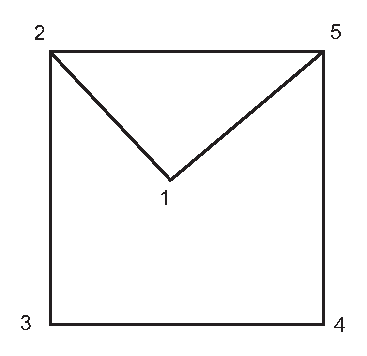
\includegraphics{\ps/no4circuit.eps}
  \caption{A $4$-circuit}
  \label{fig:no4circuit}
\end{figure}

Suppose that $D$ is a centered packing whose associated hypermap
contains such triangular and pentagonal standard regions. Recall
that $D$ determines a set $U(D)$ of vertices in Euclidean
$3$-space of distance at most $2t_0$ from the origin, and that
each vertex $p_i$ can be realized geometrically as a point on the
unit sphere at the origin, obtained as the radial projection of
some $v_i\in U(D)$.

\begin{lemma}  One of the edges $\{v_1,v_3\}$, $\{v_1,v_4\}$ has
length less than $2\sqrt{2}$.  Both of the them have lengths less
than $3.02$. Also, $|v_1|\ge2.3$.
\end{lemma}

\begin{proof} This is Lemma~\ref{tarski:4circuit}.
\end{proof}


There are restrictive bounds on the dihedral angles of the
simplices $\{0,v_1,v_i,v_j\}$ along the edge $\{0,v_1\}$. The
quasi-regular tetrahedron has a dihedral angle of at most%
\footnote{\calc{984463800}} $1.875$.  The dihedral angles of the
simplices $\{0,v_1,v_2,v_3\}$, $\{0,v_1,v_5,v_4\}$
adjacent to it are at most%
\footnote{\calc{821707685}}  $1.63$. The dihedral angle of the
remaining simplex $\{0,v_1,v_3,v_4\}$ is at most%
\footnote{\calc{115383627}} $1.51$.   This leads to lower bounds
as well. The quasi-regular tetrahedron has a dihedral angle that
is at least $2\pi - 2(1.63)-1.51 > 1.51$.  The dihedral angles
adjacent to the quasi-regular tetrahedron is at least $2\pi-
1.63-1.51-1.875> 1.26$. The remaining dihedral angle is at least
$2\pi-1.875-2(1.63) > 1.14$.

A centered packing $D$ determines a set of vertices $U(D)$ that
are of distance at most $2t_0$ from the center of $D$.  Three
consecutive vertices $p_1$, $p_2$, and $p_3$ of a standard region
are determined as the projections to the unit sphere of three
corners $v_1$, $v_2$, and $v_3$, respectively in $U(D)$. By
Lemma~\ref{lemma:1.32}, if the interior angle of the standard
region is less than $1.32$, then $|v_1-v_3|\le\sqrt{8}$.

\begin{lemma} \label{lemma:11.16}
These two standard regions $F=\{R_1,R_2\}$ give
    $\tau_F(D) \ge 11.16\,\pt$.
\end{lemma}

\begin{proof}
Let $\dih$ denote the dihedral angle of a simplex along a given
edge. Let $S_{ij}$ be the simplex $\{0,v_1,v_i,v_j\}$, for
$(i,j)=(2,3),(3,4), (4,5),(2,5)$. We have $\sum_{(4)}\dih(S_{ij})
= 2\pi$. Suppose one of the edges $\{v_1,v_3\}$ or $\{v_1,v_4\}$ has
length $\ge2\sqrt2$. Say $\{v_1,v_3\}$.

We have\footnote{\calc{572068135}, \calc{723700608},
\calc{560470084}, and \calc{535502975}}
    $$
    \begin{array}{lll}
    \tau(S_{25}) &- 0.2529\dih(S_{25}) > -0.3442,\\
    \tau_0(S_{23}) &- 0.2529\dih(S_{23}) > -0.1787,\\
    \hat\tau(S_{45}) &- 0.2529\dih(S_{45}) > -0.2137,\\
    \tau_0(S_{34}) &- 0.2529\dih(S_{34}) > -0.1371.\\
    \end{array}
    $$
We have a penalty $\xiG$ for erasing, so that
    $$
    \begin{array}{lll}
        \tau(D) &\ge \sum_{(4)}\tau_x(S_{ij}) - 5\xiG\\
                &>2\pi(0.2529)-0.3442\\
                &\qquad -0.1787-0.2137-0.1371-5\xiG\\
                &>11.16\,\pt,
    \end{array}
    $$
where $\tau_x=\tau,\hat\tau,\tau_0$ as appropriate.

Now suppose $\{v_1,v_3\}$ and $\{v_1,v_4\}$ have length $\le2\sqrt2$.
If there is an upright diagonal that is not enclosed over either
flat quarter, the penalty is at most $3\xiG+2\xiV$. Otherwise, the
penalty is smaller: $4\xiG'+\xiV$. We have
    $$
    \begin{array}{lll}
    \tau(D)
    &\ge \sum_{(4)}\tau(S_{ij})-(3\xiG+2\xiV)\\
    &>2\pi(0.2529)-0.3442\\
    &\qquad -2(0.2137)-0.1371 -(3\xiG+2\xiV)\\
    &>11.16\,\pt.\\
    \end{array}
    $$
\end{proof}



\section{mixed bound} %DCG 10.14, p105 (moved -1.04 bound)
% Rewritten.

\begin{lemma} \label{lemma:1.04}
%\proclaim{Proposition 4.1}
The score of a mixed quad cluster is less than $-1.04\,\pt$.
\end{lemma}

\begin{proof}
In a mixed quad cluster there is at least one enclosed vertex.
Any enclosed vertex in a quad cluster has length at least $2t_0$
by Lemma~\ref{lemma:enclosed}. In particular, the anchors of an
enclosed vertex are corners of the quad cluster. There are no flat
quarters.

We erase all of the enclosed vertices except for one, which
we can do with the estimate of Lemma~\ref{lemma:mixed-vor0}.
The enclosed vertex has zero, one, or two anchors.  The upright
quarters around that vertex are scored with the function appropriate
to its context.
The rest of the quad cluster is estimated by the function $\vor_0$.

If the enclosed vertex has zero anchors, then the entire quad
cluster $(R,D)$ satisfies $$\sigma_R(D)\le \vor_{0,R}(D).$$
The right-hand side of this equation is independent of the enclosed
vertex $v$.  In particular, we can move it until 
two consecutive  corners of the quad cluster are anchors of $\{0,v\}$
and one of the distances $|v-v_i|=2.51$ for one of those two corners.

A calculation shows%
\footnote{\calc{XX}. This is a new interval calculation that
needs to be verified: If $(R,D)$ is any quad cluster with both
diagonals greater than $\sqrt8$, and some distance $|v_i-v_{i+1}|>2.38$,
then $\vor_{0,R}(D) < -1.04\,\pt$.} 
that if $\sigma_R(D) \ge -1.04\,\pt$, then 
$|v_i-v_{i+1}|\le 2.38$ for $i=1,2,3,4$.  We assume these
constraints.

We may use the deformation of Lemma~\ref{x-4.9.2}
at each vertex $v_i$ that is not an anchor of $\{0,v\}$ so either
it becomes an anchor (with $|v-v_i|=2t_0$), or it satisfies
  $$|v_i-v_{i+1}|=|v_i-v_{i-1}|=2;\quad |v_i|\in\{2,2t_0\}.$$ 

In the course of deformation (say of corner $v_1$),  
the diagonal $\{v_1,v_3\}$ may reach length $\sqrt8$.  
In this case, we stop
the deformation at that corner and continue with another
corner (say $v_2$, if it exists)
that is not an anchor until its deformation
is complete, and then return to the complete the deformation
at $v_1$.  We cannot have both diagonals $\{v_1,v_3\}$ and $\{v_2,v_4\}$
drop to $\sqrt8$, by Lemma~\ref{XX:tarski}, unless $\{0,v\}$ has four
anchors.  The result, after the deformations are complete, may
have a diagonal of length less than $\sqrt8$.  At this point,
that constraint is no longer needed.  Its only purpose was to
fulfill a hypothesis of Lemma~\ref{x-4.9.2}.

We claim that if corner $v_i$ is not an anchor of $\{0,v\}$,
then $2t_0 < |v-v_i| \le 2.95$.  In fact, if $|v-v_i| > 2.96$,
then the sum of the dihedral angles around $\{0,v\}$ satisfies%
\footnote{\calc{XX}.  These are new interval calculations 
  that need to be verified.  For an upright quarter in
  $[2.51,\sqrt8][2,2.51]^2[2,2.38][2,2.51]^2$, $\dih < 2.01$.
For a simplex in $[2.51,\sqrt8][2,2.51]^2 [2] [2.96,++][2,++]$,
$\dih < 1.13$.}
 $$
 2\pi = \sum_{i=1}^4 \dih_V(\{0,v\},\{v_i,v_{i+1}\}) < 2(2.01)+2(1.13) < 2\pi.
 $$

We write the upper bound on $\sigma_R(D)$ 
as a sum of contributions from the four simplices
$\{0,v,v_i,v_{i+1}\}$.    That contribution is the score of the
upright quarter, if the simplex is an upright quarter in the $Q$-system.
Otherwise, we use the upper bound $\vor_0$.

If $\{0,v\}$ has just two anchors (say at adjacent corners $v_1,v_4$),
then the contribution from $\{0,v,v_1,v_4\}$ is at most $0$.  In
fact, if the simplex is an upright quarter in the $Q$-system, this
follows from Lemma~\ref{XX}.  If the simplex is scored by $\vor_0$,
then (say) $|v-v_1|=2t_0$ and the result is a calculation.%
\footnote{\calc{XX}.  This is a new calculation.  
It needs to be verified.  If an upright
simplex satisfies $[2.51,\sqrt8][2,2.51]^2[2,2.38][2.51][2,2.51]$,
then $\vor_0(S) < 0$.}  Moreover, the contributions from the other
three simplices give%
\footnote{\calc{XX}. These are new calculations.  They need
to be verified.  On
$[2.51,\sqrt8]\{2,2.51\}^2[2][2.51,2.96]^2$, $\vor_0 < -0.0475$; and
on $[2.51,\sqrt8]\{2,2.51\}[2,2.51][2][2.51,2.96][2,2.51]$,
   $\vor_0 < -0.0055$.
}
 $$\sum_{i=1}^3\vor_{0,R,V}(0,\{v,v_i,v_{i+1}\}) <
   -0.0055 - 0.0475 - 0.0055 < -1.04\,\pt.$$

If $\{0,v\}$ has three anchors (say $v_1,v_2,v_4$), then
writing $\sigma'_i$ for the upper bound on the contribution
from $\{0,v,v_i,v_{i+1}\}$, we have%
\footnote{\calc{XX}.  These are new calculations that need to
be verified.  For an upright quad with $y_4\in[2,2.38]$, we
have $\sigma(Q) < \epsilon_1 -0.08(\dih(Q)-\pi/2)$.  I added
this small $\epsilon_1$ to make it more likely that it will follow
by a linear program for the other inequalities for $\sigma(Q)$.
Note that there are various cases, according to the context; we
haven't erased anything here.  We have the similar
  $\vor_0 < \epsilon_1 -0.08(\dih(Q)-\pi/2)$,
when $[2.51,\sqrt8][2,2.51]^2[2,2.38][2,2.51][2.51]$.  Then we
have $\vor_0 < \epsilon_2  -0.08(\dih(Q)-\pi/2)$,
when $[2.51,\sqrt8][2,2.51]^2[2][2,2.51][2.51,2.96]$.
}
  $$
  \sum_{i=1}^4\sigma'_i < 
  \sum (\epsilon_i -0.08 (\dih_V(\{0,v\},\{v_i,v_{i+1}\})-\pi/2))
  = \sum\epsilon_i = -1.04\,\pt.
  $$
where $\epsilon_2=\epsilon_3 = -0.54\,\pt$ and $\epsilon_1=\epsilon_4 =
0.02\,\pt$.
\end{proof}

%% OLD PROOF. 
%
%We generally truncate the $V$-cell at $\sqr2$ as in the proof of
%Theorem~\ref{lemma:quad0}.  By that lemma, it breaks the $V$-cell
%into pieces whose score is nonpositive. Thus, if we identify
%certain pieces that score less than $-1.04\,\pt$, the result
%follows. Nevertheless, a few simplices will be left untruncated in
%the following argument. We will leave a simplex untruncated only
%if we are certain that this is justified.
%%% Avoid mention of orien-tation.
%% Each of its faces has positive orien-tation
%% and that the simplices sharing a face $F$ with $S$ either lie in
%% the $Q$-system or have positive orien-tation along $F$.  
%If so, we may use\footnote{\calc{185703487},
%\calc{69785808}, and \calc{104677697}} the function $\svor$ on $S$
%rather than truncation $\svor_0$.
%
%In this proof, by enclosed vertex, we mean one of height at most
%$2\sqrt2$. Let $v$ be an enclosed vertex with the fewest anchors.
%If there are no anchors, the right circular cone $C(h,\eta_0(h))$
%(aligned along $\{0,v\}$; see Definition~\ref{def:cone}) belongs
%to $\op{VC}(0)$, where $\eta_0(h)=\eta(2h,2,2t_0)$ as in
%Definition~\ref{def:eta0} and $|v|=2h$. In fact, if such a point
%lies in $\op{VC}(u)$, with $u \ne v$, then $u$ must be a corner of
%the quad cluster or an enclosed vertex of height at least $2t_0$.
%In either case, the right circular cone belongs to $\op{VC} (0)$.
%By Formula~\ref{eqn:3.2}, the score of this cone is
%$2\pi(1-h/\eta_0(h))\phi(h,\eta_0(h))$. An optimization in one
%variable gives an upper bound of $-4.52\,\pt$, for $t_0\le h\le
%\sqr2$.   This gives the bound of $-1.04\,\pt$ in this case.
%
%If there is one anchor,  we cut the cone in half along the plane
%through $\{0,v\}$ perpendicular to the plane containing the anchor
%and $\{0,v\}$. The half of the cone on the far side of the anchor
%lies under the face at $v$ of the $V$-cell.  We get a bound of
%$-4.52\,\pt/2 < -1.04\,\pt$.
%
%In the remaining cases, each enclosed vertex has at least two
%anchors.  Each anchor is a corner of the quad cluster.  Fix an
%enclosed vertex $v$. Suppose that $v_1$, a corner, is an anchor of
%$v$. Assume that the face $\{0,v,v_1\}$ bounds at most one upright
%quarter. We sweep around the edge $\{0,v_1\}$, away from the
%upright quarter if there is one,  until we come to another
%enclosed vertex $v'$ such that $\{0,v_1,v'\}$ has circumradius
%less than $\sqr2$ or such that $v_1$ is an anchor of $\{0,v'\}$.
%If such a vertex $v'$ does not exist, we sweep all the way to
%$v_2$ a corner of the quad cluster adjacent to $v_1$.
%
%Section~\ref{sec:K} defines a function $K$ that we use in
%this proof.
%
%If $v'$ exists, then various
%calculations\footnote{\calc{104677697}, \calc{69785808},
%\calc{586706757}, and \calc{87690094}} give the bound
%$-1.04\,\pt$, depending on the size of the circumradius of
%$\{0,v,v'\}$. This allows us to assume that we do not encounter
%such an enclosed vertex $v'$ whenever we sweep away, as above,
%from the face formed by an anchor.
%
%Now consider the simplex $S=\{0,v_1,v_2,v\}$, where $v_1$ is an
%anchor of $\{0,v\}$.  We assume that it is not an upright quarter.
%There are three alternatives. The first is that $S$ decreases the
%score of the quarter by at least $0.52\,\pt$.
%Calculations\footnote{\calc{185703487} and \calc{441195992}} show
%that this occurs if the circumradius of the face $\{0,v,v_2\}$ is
%less than $\sqr2$, or if the circumradius of the face is greater
%than $\sqr2$, provided that the length of $\{v,v_1\}$ is at most
%$2.2$. The second alternative\footnote{\calc{848147403},
%\calc{969320489}, and \calc{975496332}.} is that the face
%$\{0,v,v_1\}$ of $S$ is shared with a quarter $Q$ and that $S$ and
%$Q$ taken together bring the score down by $0.52\,\pt$. In fact,
%if there are two such simplices $S$ and $S'$ along $Q$, then the
%three simplices $Q$, $S$, and $S'$ pull the
%score\footnote{\calc{766771911}} below $-1.04\,\pt$. The third
%alternative is that there is a simplex $S'=\{0,v,v,v_3\}$ sharing
%the face $\{0,v,v_1\}$, which, like $S$, scores less than
%$-0.31\,\pt$.  In each case, $S$ and the adjacent simplex through
%$\{0,v,v_1\}$ score less than $-0.52\,\pt$. Since $v$ has at least
%two anchors, the quad cluster scores less than $2(-0.52)\,\pt
%=-1.04\,\pt$.
%%
%
%



\section{A particular $5$-circuit} %DCG 14.3, p160

\begin{lemma}\label{lemma:6079}  Assume that $R$ is a pentagonal standard region
    with an enclosed vertex $v$ of height at most $2t_0$.
    %(See Figure~\ref{fig:pent-tri1}.)
    Assume further that
    \begin{itemize}
        \item $|v_i|\le 2.168$ for each of the five corners.
        \item Each interior angle of the pentagon is at most
        $2.89$.
        \item If $v_1$, $v_2$, $v_3$ are consecutive corners over
        the pentagonal region, then $$|v_1-v_2|+|v_2-v_3|<4.804.$$
        \item $\sum_5 |v_i-v_{i+1}|\le 11.407.$
    \end{itemize}
    Then $\sigma_R(D)< -0.2345$ or $\tau_R(D) > 0.6079.$
\end{lemma}

\begin{proof}
Since $-0.4339$ is less than this the lower bound, a $3$-crowded
upright diagonal does not occur. Similarly, since $-0.25$ is less
than the lower bound, a $4$-crowded upright diagonal does not
occur (Lemma~\ref{lemma:4-crowded} and Lemma~\ref{x-3.8}).

Suppose that there is a loop in context $(n,k)=(4,2)$. Again by
Lemma~\ref{lemma:loop} (with $n(R)=7$),
$$\sigma_R(D)  < -0.2345.$$
%The constants come from
%Table~\ref{x-5.11} and  Theorem~\ref{thm:the-main-theorem}.

%If we branch and bound on the triangular faces, this LP-derived
%inequality can be improved to
%    $$\tau[F] < 0.6079.$$

%If there is a loop other than $(4,2)$ and $(4,1)$, the linear
%program becomes infeasible:
%    $$\tau[F] < 0.644 < t_7 + \dloop(n,k) < \tau[F].$$
We conclude that all loops have context $(n,k)=(4,1)$.


{\bf Case 1.}  {\it The vertex $v=v_{12}$ has distance at least
$2t_0$ from the five corners of $U(D)$ over the pentagon.}

%The interval calculations relevant in Case 1 appear in
%~\ref{A.3.8}.

The penalty to switch the pentagon to a pure $\vor_0$ score is at
most $5\xiG$ (see Section~\ref{sec:prep-cluster}).  There cannot
be two flat quarters because then Lemma~\ref{tarski:E:part4:5} gives
$$|v_{12}|>2t_0.$$


{\bf (Case 1-a)} Suppose there is one flat quarter,
$|v_1-v_4|\le2\sqrt2$. There is a lower bound of 1.2 on the
dihedral angles of the simplices $\{0,v_{12},v_i,v_{i+1}\}$.  This
is obtained as follows.  The proof relies on the convexity of the
quadrilateral region.  We leave it to the reader to verify that
the following pivots can be made to preserve convexity.  Disregard
all vertices except $v_1,v_2,v_3,v_4,v_{12}$.  We give the
argument that $\dih(0,v_{12},v_1,v_4)>1.2$.  The others are
similar. Disregard the length $|v_1-v_4|$.  We show that
    $$
    \begin{array}{lll}
        sd &:=\dih(0,v_{12},v_1,v_2)+\dih(0,v_{12},v_2,v_3)\\
           &+\dih(0,v_{12},v_3,v_4) < 2\pi-1.2.
    \end{array}
    $$
Lift $v_{12}$ so $|v_{12}|=2t_0$. Maximize $sd$ by taking
$|v_1-v_2|=|v_2-v_3|=|v_3-v_4|=2t_0$.  Fixing $v_3$ and $v_4$,
pivot $v_1$ around $\{0,v_{12}\}$ toward $v_4$, dragging $v_2$
toward $v_{12}$ until $|v_2-v_{12}|=2t_0$.  Similarly, we obtain
$|v_3-v_{12}|=2t_0$. We now have $sd\le 3(1.63)< 2\pi-1.2$, by a
calculation.\footnote{\calc{821707685}}

Return to the original figure and move $v_{12}$ without increasing
$|v_{12}|$ until each simplex $\{0,v_{12},v_i,v_{i+1}\}$ has an edge
$(v_{12},v_j)$ of length $2t_0$. Interval
calculations\footnote{\calc{467530297} and \calc{135427691}} show
that the four simplices around $v_{12}$ squander
    $$2\pi(0.2529)-3(0.1376)-0.12 > \squander + 5\xiG.$$

{\bf (Case 1-b)} Assume there are no flat quarters. By hypothesis,
the perimeter satisfies $$\sum|v_i-v_{i+1}|\le 11.407.$$ We have
$\arc(2,2,x)'' = 2x/(16-x^2)^{3/2} >0$. The arclength of the
perimeter is therefore at most
$$2\arc(2,2,2t_0) + 2\arc(2,2,2) + \arc(2,2,2.387) <  2\pi.$$
There is a well-defined interior of the spherical pentagon, a
component of area $<2\pi$.  If we deform by decreasing the
perimeter, the component of area $<2\pi$ does not get swapped with
the other component.

Disregard all vertices but $v_1,\ldots,v_5,v_{12}$.  If a vertex
$v_i$ satisfies  $|v_i-v_{12}|>2t_0$, deform $v_i$ as in
Section~\ref{x-4.9} until $|v_{i-1}-v_{i}|=|v_i-v_{i+1}|=2$, or
$|v_i-v_{12}|=2t_0$. If at any time, four of the edges realize the
bound $|v_i-v_{i+1}|=2$, we have reached an impossible situation,
because it leads to the contradiction\footnote{\calc{115383627}
and \calc{603145528}}
    $$2\pi = \sum^{(5)}\dih < 1.51 + 4 (1.16) < 2\pi.$$
(This inequality relies on the observation, which we leave to the
reader, that in any such assembly, pivots can by applied to bring
$|v_{12}-v_i|=2t_0$ for at least one edge of each of the five
simplices.)



The vertex $v_{12}$ may be moved without increasing $|v_{12}|$ so
that eventually by these deformations (and reindexing if
necessary) we have $|v_{12}-v_i|=2t_0$, $i=1,3,4$. (If we have
$i=1,2,3$, the two dihedral angles along $\{0,v_2\}$
satisfy\footnote{\calc{115383627}} $<2(1.51)<\pi$, so the
deformations can continue.)



There are two cases. In both cases $|v_i-v_{12}|=2t_0$, for
$i=1,3,4$.
$$
\begin{array}{lll}
(i)\quad &|v_{12}-v_2|=|v_{12}-v_5|=2t_0,\\
(ii)\quad &|v_{12}-v_2|=2t_0,\quad |v_4-v_5|=|v_5-v_1|=2,\\
\end{array}
$$
Case (i) follows from interval
calculations\footnote{\calc{312132053}}
$$
\sum\tau_0 \ge 2\pi(0.2529) - 5 (0.1453) > 0.644+7\xiG.
$$
In case (ii), we have again
    $$2\pi(0.2529)-5 (0.1453).$$
In this interval calculation we have assumed that
$|v_{12}-v_5|<3.488$. Otherwise, setting $S=(v_{12},v_4,v_5,v_1)$, Lemma~\ref{tarski:3488}
shows the simplex does not exist.
($|v_4-v_1|\ge2\sqrt2$ because
there are no flat quarters.)
This completes Case 1.

\medskip

{\bf Case 2.} {\it The vertex $v_{12}$ has distance at most $2t_0$
from the vertex $v_1$ and distance at least $2t_0$ from the
others.}

Let $\{0,v_{13}\}$ be the upright diagonal of a loop $(4,1)$.  The
vertices of the loop are not $\{v_2,v_3,v_4,v_5\}$ with $v_{12}$
enclosed over $\{0,v_2,v_5,v_{13}\}$ by
Lemma~\ref{lemma:anc-simplex-not-enc}. The vertices of the loop
are not $\{v_2,v_3,v_4,v_5\}$ with $v_{12}$ enclosed over
$\{0,v_1,v_2,v_5\}$ because this and Lemmas~\ref{tarski:E:part4:6}
and \ref{tarski:E:part4:7} would lead to a contradiction
$y_{12}>2t_0$. 
We get a contradiction for the same reasons
 unless $\{v_1,v_{12}\}$ is an edge of some
upright quarter of every loop of type $(4,1)$.

We consider two cases.  (2-a) There is a flat quarter along an
edge other than $\{v_1,v_{12}\}$.  That is, the central vertex is
$v_2$, $v_3$, $v_4$, or $v_5$.  (Recall that the {\it central
vertex} of a flat quarter is the vertex other than the origin that
is not an endpoint of the diagonal.) (2-b) Every flat quarter has
central vertex $v_1$.

{\bf Case 2-a.}  We erase all upright quarters including those in
loops, taking penalties as required. There cannot be two flat
quarters because then Lemmas~\ref{tarski:E:part4:8} and
\ref{tarski:E:part4:9} would imply $|v_{12}|>2t_0$.

The penalty is at most $7\xiG$.  We show that the region (with
upright quarters erased) squanders $>7\xiG+0.644$.  We assume that
the central vertex is $v_2$ (case 2-a-i) or $v_3$ (case 2-a-ii).
In case 2-a-i, we have three types of simplices around $v_{12}$,
characterized by the bounds on their edge lengths.  Let
$\{0,v_{12},v_1,v_5\}$ have type A, $\{0,v_{12},v_5,v_4\}$ and
$\{0,v_{12},v_4,v_3\}$ have type B, and let $\{0,v_{12},v_3,v_1\}$
have type C.  In case 2-a-ii there are also three types.  Let
$\{0,v_{12},v_1,v_2\}$ and $\{0,v_{12},v_1,v_5\}$ have type A,
$\{0,v_{12},v_5,v_4\}$ type B, and $\{0,v_{12},v_2,v_4\}$ type D.
(There is no relation here between these types and the types of
simplices $A$, $B$, $C$ defined in \Chap~\ref{sec:fine}.) Upper
bounds on the dihedral angles along the edge $\{0,v_{12}\}$ are
given as calculations\footnote{\calc{821707685}, \calc{115383627},
\calc{576221766}, and \calc{122081309}}. These upper bounds come
as a result of a pivot argument similar to that establishing the
bound 1.2 in Case 1-a.

These upper bounds imply the following lower bounds.  In case
2-a-i,
$$
\begin{array}{lll}
\dih &> 1.33 \quad(A),\\
\dih &> 1.21 \quad(B),\\
\dih &> 1.63 \quad(C),\\
\end{array}
$$
and in case 2-a-ii,
$$
\begin{array}{lll}
\dih &> 1.37 \quad(A),\\
\dih &> 1.25 \quad(B),\\
\dih &> 1.51 \quad(D),\\
\end{array}
$$
In every case the dihedral angle is at least $1.21$. In case
2-a-i, the inequalities give a lower bound on what is squandered
by the four simplices around $\{0,v_{12}\}$. Again, we move $v_{12}$
without decreasing the score until each simplex
$\{0,v_{12},v_i,v_{i+1}\}$ has an edge satisfying
$|v_{12}-v_j|\le2t_0$. Interval
calculations\footnote{\calc{644534985}, \calc{467530297}, and
\calc{603910880}} give
    $$
    \begin{array}{lll}
    \sum_{(4)}\tau_0 &> 2\pi (0.2529) - 0.2391-2(0.1376)-0.266\\
        &>0.808.
    \end{array}
    $$
In case 2-a-ii, we have\footnote{\calc{135427691}}
    $$
    \begin{array}{lll}
    \sum_{(4)}\tau_0 &> 2\pi (0.2529) - 2(0.2391)-0.1376-0.12\\
        &>0.853.
    \end{array}
    $$
So we squander more than $7\xiG+0.644$, as claimed.

{\bf Case 2-b.}  We now assume that there are no flat quarters
with central vertex $v_2,\ldots,v_5$. We claim
 that $v_{12}$ is not enclosed over $\{0,v_1,v_2,v_3\}$ or
$\{0,v_1,v_5,v_4\}$. In fact, if $v_{12}$ is enclosed over
$\{0,v_1,v_2,v_3\}$, then we reach the
contradiction\footnote{\calc{821707685} and \calc{115383627}}
    $$
    \begin{array}{lll}
    \pi&<\dih(0,v_{12},v_1,v_2)+\dih(0,v_{12},v_2,v_3)\\
        &< 1.63+1.51 < \pi.
    \end{array}
    $$

We claim
 that $v_{12}$ is not enclosed over $\{0,v_5,v_1,v_2\}$.
Let $S_1=\{0,v_{12},v_1,v_2\}$, and $S_2=\{0,v_{12},v_1,v_5\}$.  We
have by hypothesis,
$$y_4(S_1)+y_4(S_2) = |v_1-v_2|+|v_1-v_5|< 4.804.$$
An interval calculation\footnote{\calc{69064028}} gives
    $$
    \begin{array}{lll}
    \sum_{(2)}\dih(S_i) &\le \sum_{(2)}
    \left(\dih(S_i)+0.5(0.4804/2-y_4(S_i))\right)\\
    &<\pi.
    \end{array}
    $$
So $v_{12}$ is not enclosed over $\{0,v_1,v_2,v_5\}$.

Erase all upright quarters, taking penalties as required.  Replace
all flat quarters with $\svor_0$-scoring taking penalties as
required. (Any flat quarter has $v_1$ as its central vertex.) We
move $v_{12}$ keeping $|v_{12}|$ fixed and not decreasing
$|v_{12}-v_1|$.  The only effect this has on the score comes
through the quoins along $\{0,v_1,v_{12}\}$. Stretching
$|v_{12}-v_1|$ shrinks the quoins and increases the score. (The
sign of the derivative of the quoin with respect to the top edge
is computed in the proof of Lemma~\ref{x-4.9.1}.)

If we stretch $|v_{12}-v_1|$ to length $2t_0$, we are done by case
1 and case 2-a. (If deformations produce a flat quarter, use case
2-a, otherwise use case 1.) By the claims, we can eventually
arrange (reindexing if necessary) so that
$$
\begin{array}{lll}
(i)&\quad |v_{12}-v_3|=|v_{12}-v_4|=2t_0,\quad\text{or}\\
(ii)&\quad |v_{12}-v_3|=|v_{12}-v_5|=2t_0.
\end{array}
$$
We combine this with the deformations of Section~\ref{x-4.9} so
that in case (i) we may also assume that if $|v_5-v_{12}|>2t_0$,
then $|v_4-v_5|=|v_5-v_1|=2$ and that if $|v_2-v_{12}|>2t_0$, then
$|v_1-v_2|=|v_2-v_3|=2$. In case (ii) we may also assume that if
$|v_4-v_{12}|>2t_0$, then $|v_3-v_4|=|v_4-v_5|=2$ and that if
$|v_2-v_{12}|>2t_0$, then $|v_1-v_2|=|v_2-v_3|=2$.

Break the pentagon into subregions by cutting along the edges
$(v_{12},v_i)$ that satisfy $|v_{12}-v_i|\le2t_0$. So for example
in case (i), we cut along $(v_{12},v_3)$, $(v_{12},v_4)$,
$(v_{12},v_1)$, and possibly along $(v_{12},v_2)$ and
$(v_{12},v_5)$.  This breaks the pentagon into triangular and
quadrilateral regions.

In case (ii), if $|v_4-v_{12}|>2t_0$, then the argument used in
Case 1 to show that $|v_4-v_{12}|<3.488$ applies here as well.
%% Keep comment: DCG p164.  I commented out to avoid mention of Delta.
%% But it is used eventually in the argument.
%% Deelta doesn't explicitly get mentioned in the two footnoted calcs,
%% so what I'm commented out isn't that essential.
% In
%case (i) or (ii), if $|v_{12}-v_2|>2t_0$, then for similar
%reasons, we may assume
%    $$\Deelta(|v_{12}-v_2|^2,4,4,8,(2t_0)^2,|v_{12}-v_1|^2)\ge0.$$
We use
calculations\footnote{\calc{312132053} and \calc{644534985}} to
conclude that
    $$\sum\tau_0 \ge 2\pi (0.2529) -3 (0.1453) -2 (0.2391) > 0.6749.$$
If the penalty is less than $0.067=0.6749-0.6079$, we are done.

We have ruled out the existence of all loops except $(4,1)$. Note
that a flat quarter with central vertex $v_1$ gives penalty at
most $0.02$ by Lemma~\ref{x-3.11.3}.
  If there is at most one
such a flat quarter and at most one loop, we are done:
$$3\xiG + 0.02 < 0.067.$$
Assume there are two loops of context $(n,k)=(4,1)$.  They both
lie along the edge $\{v_1,v_{12}\}$, which precludes any unmasked
flat quarters. If one of the upright diagonals has height
$\ge2.696$, then the penalty is at most $3\xiG+3\xiV< 0.067$.
Assume both heights are at most $2.696$. The total interior angle
of the exceptional face at $v_1$ is at least four times the
dihedral angle of one of the flat quarters along $\{0,v_1\}$, or
$4(0.74)$ by an interval calculation\footnote{\calc{751442360}}. This is
contrary to the hypothesis of an interior angle $<2.89$.   This
completes Case 2. This shows that heptagons with pentagonal hulls
do not occur.
\end{proof}

\begin{lemma}\label{lemma:excess-1}
Let $R$ be an exceptional standard region.  Let $V$
be a set of vertices of $R$.  If $v\in V$, let $p_v$ be the number
of triangular regions at $v$ and let $q_v$ be the number of
quadrilateral regions at $v$.  Assume that $V$ has the following
properties:
    \begin{enumerate}
        \item No two
        vertices in $V$ are adjacent.
        \item No two vertices
        in $V$ lie on a common quadrilateral.
        \item If $v\in V$, then there are five standard regions at
        $v$.
        \item If $v\in V$, then the corner over $v$ is a central
        vertex of a flat quarter in the cone over $R$.
        \item If $v\in V$, then $p_v\ge 3$.  That is, at least
        three of the five standard regions at $v$ are triangular.
        \item If $R'\ne R$ is an exceptional region at $v$, and if $R$
        has interior angle at least $1.32$ at $v$, then $R'$ also has interior
        angle at least $1.32$ at $v$.
        \item If $(p_v,q_v)=(3,1)$, then the internal angle at $v$ of the exceptional
        region is at most $1.32$.
    \end{enumerate}
  Define $a:\N\to \R$ by
  $$a(n) = \begin{cases}
    14.8 &n=0,1,2,\\
    1.4 & n=3,\\
    1.5 & n=4,\\
    0 & \text{otherwise.}
  \end{cases}
  \index{aZ@$a(n)$}
  $$
Let $\{F\}$ be the union of $\{R\}$ with the set of triangular and
quadrilateral regions that have a vertex at some $v\in V$. Then
    $$\sum_F\tau_F(D) > \sum_{v\in V} (p_v d(3) + q_v d(4) + a
    (p_v))\,\pt.$$
\end{lemma}

\begin{proof}   We erase all upright diagonals in the
$Q$-system, except for those that carry a penalty: loops,
$3$-unconfined, $3$-crowded, and $4$-crowded diagonals.

We assume that if $(p_v,q_v)=(3,1)$, then the internal angle is at
most $1.32$. Because of this, if we score the flat quarter by
$\vor_0$, then the flat quarter $Q$ satisfies
(Lemma~\ref{lemma:1.32})
   \begin{equation}
   \vor_0(Q) > 3.07\,\pt > 1.4\,\pt + D(3,1) + 2\xiV + \xiG.
   \label{eqn:307}
   \end{equation}



Every flat quarter that is masked by a remaining upright quarter
in the $Q$-system has $y_4\ge2.6$.  Moreover, $y_1\ge2.2$ or
$y_4\ge2.7$.  Let $\pi_v = 2\xiV + \xiG$ if the flat quarter is
masked, and $\pi_v = 0$ otherwise.

We claim that the flat quarter (scored by $\vor_0$) together with
the triangles and quadrilaterals at a given vertex $v$ squander at
least
   \begin{equation}
   (p_v d(3) + q_v d(4) + a(p_v))\,\pt + D(3,1) + \pi_v
   \label{eqn:one-v}
   \end{equation}
If $p_v=4$, this is \calc{314974315}.  If $p_v=3$, we may assume
by the preceding remarks that there are two exceptional regions at
$v$.  If the internal angle of $R$ at $v$ is at most $1.32$, then
we use Inequality~\ref{eqn:307}.  If the angle is at least $1.32$,
then by hypothesis, the angle $R'$ at $v$ is at least $1.32$.  We
then appeal to the calculations \calc{675785884} and
\calc{193592217}.

To complete the proof of the lemma, it is enough to show that we
can erase the upright quarters masking a flat quarter at $v$
without incurring a penalty greater than $\pi_v$.  For then, by
summing the Inequality~\ref{eqn:one-v} over $v$, we obtain the
result.

If the upright diagonal is enclosed over the masked flat quarter,
then the upright quarters can be erased with penalty at most
$\xiV$ (by Remark~\ref{remark:3rd-quarter}). Assume the upright
diagonal is not enclosed over the masked flat quarter.

If there are at most three upright quarters, the penalty is at
most $2\xiV + \xiG$.  Assume four or more upright quarters.  If
the upright diagonal is not a loop, then it must be $4$-crowded.
This can be erased with penalty
   $$2\xiV + 2\xiG - \kappa < 2\xiV + \xiG.$$

Finally, assume that the upright quarter is a loop with four or
more upright quarters.  Lemma~\ref{lemma:loop} limits the
possibilities to parameters $(5,0)$ or $(5,1)$.  In the case of a
loop $(5,1)$, there is no need to erase because $|V|\le3$ and by
Lemma~\ref{lemma:loop}, the hexagonal standard region squanders at
least
   $$t_6 + 3 a(p_v)\,\pt$$
as required by the lemma.  In the case of a loop $(5,0)$ in a
pentagonal region, if $|V|=1$ then there is no need to erase
(again we appeal to Lemma~\ref{lemma:loop}).  If $|V| =2$, then
the two vertices share a penalty of $4\xiV + \xiG$, with each
receiving
   $$2\xiV + \xiG/2 < 2\xiV +\xiG.$$
\end{proof}
